% Dokumenteneinstellungen
\documentclass[a4paper,abstracton,DIV=classic,11pt]{scrreprt}

\usepackage[utf8]{inputenc}
\usepackage[T1]{fontenc}
\usepackage[english]{babel}

% Schriftart und Darstellung
\usepackage{xcolor}
\definecolor{eumetsatblau}{HTML}{00205b}

\usepackage{flafter}
\usepackage{mathpazo}
\usepackage{microtype}
\usepackage{graphicx}
\addtokomafont{disposition}{\rmfamily\color{eumetsatblau}} % Überschriften auch mit Serifen
\usepackage{booktabs}
\usepackage{multirow}
\usepackage[artemisia]{textgreek}

% Seitenkopf- und Fußzeilen
\usepackage{lastpage}

% scrlayer-scrpage Paket für Kopf- und Fußzeilen
\usepackage[headsepline]{scrlayer-scrpage}
\addtokomafont{headsepline}{\color{eumetsatblau}}
\addtokomafont{footsepline}{\color{eumetsatblau}}

% Kopf- und Fußzeilenstile definieren
\pagestyle{scrheadings}
\ihead{\rightmark} \chead[]{} \ohead[\pagemark]{\pagemark} 
\cfoot[]{}
\renewcommand{\headfont}{\rmfamily \color{eumetsatblau}}
\automark{chapter} 

% Paket für Einheiten
\usepackage{siunitx}
\DeclareSIUnit\dbZ{dBZ}
\sisetup{
    detect-mode=false,
    mode=text,
}

% Titelseitenangaben
\title{Associate Scientist Activity for the validation of the Convection Initiation (CI) product of NWC\,SAF v2018}
\author{Stephan Lenk, Fabian Senf, Hartwig Deneke}
\subtitle{Associate Scientist Activity conducted at Nowcasting Departement of M\'{e}t\'{e}o-France, Toulouse, France}
\subject{Final Report on the}
\date{Period May-August 2018} 

% Zitierstil
\usepackage{natbib}
\bibliographystyle{ametsoc2014}  

% Literature statt Biliography
\addto\captions{\renewcommand{\refname}{Literature}}
\renewcommand{\bibname}{Literature}

% Abbildungen fortlaufend nummerieren
\usepackage{chngcntr}
\counterwithout{figure}{chapter}
\counterwithout{table}{chapter} 
\counterwithout{equation}{chapter}
\counterwithout{footnote}{chapter}

% Pakete für Abbildungen mit mehreren Grafiken
\usepackage{caption}
\usepackage{subcaption}

% Matheumgebungspakete
\usepackage{amsmath}
\usepackage{amsfonts}
\usepackage{amssymb}

\newcommand{\marked}[1]{\textbf{#1}}

% Anteil, den Floats haben müssen, damit sie auf eine neue Seite dürfen
\renewcommand{\floatpagefraction}{.7}

% Paket für Änderungsverfolgung
\usepackage[inline]{trackchanges}
\addeditor{SL}
\addeditor{FS}
\addeditor{JMM}
\addeditor{HD}

\addto{\captionsenglish}{%
  \renewcommand{\bibname}{References}
}

% Dokument %%%%%%%%%%%%%%%%%%%%%%%%%%%%%%%%%%%%%%%%%%%%%%%%%%%%%%%%%%%%%%%%%%%%
\begin{document}

% Titelseite mit Logos aufbauen
\makeatletter
    \begin{titlepage}
        \begin{center}
        	
\includegraphics[width=0.6\linewidth]{Grafiken/Logos/eumetsat_logo.pdf} \\
        	
\includegraphics[width=0.6\linewidth]{Grafiken/Logos/nwcsaf_logo.pdf} \\[1ex]
            
\includegraphics[width=0.25\linewidth]{Grafiken/Logos/LogoMeteoFrance.pdf}\\[2ex]
            
\includegraphics[width=0.4\linewidth]{Grafiken/Logos/Schriftzug_en.pdf}\\[4ex]
            {\Large \bfseries \@author} \\[3ex]
            {\large \@subject} \\[3ex]
            {\huge \bfseries  \@title }\\[3ex] 
            {\large  \@subtitle}\\[1ex] 
            {\large \@date} \\ [2ex]
            {\large NWC\,SAF/MF-PI responsible of Activity : J.-M. Moisselin} \\ [2ex]
            {\large NWC\,SAF code of the document: NWC/CDOP3/SAF/MF-PI/SCI/RP/Ci\_Improv\_Tropos} \\ [1ex]
        \end{center}
    \end{titlepage}
\makeatother

% neue Seite und Seitennummerierung zurücksetzen
\newpage
\setcounter{page}{1}
\pagenumbering{arabic}

\renewcommand\abstractname{Executive summary}
\begin{abstract}
\addcontentsline{toc}{chapter}{Executive summary}
This report summarises the results of the analyses which have been conducted in the framework of the M\'{e}t\'{e}o France -- EUMETSAT associate scientist activity to validate the improved Convection Initiation (CI) product developed for the NWC\,SAF v2018 GEO software package.  

The detection of clouds that will develop into thunderstorms is an important but challenging task in operational weather forecast. Hence, a number of different satellite-based approaches to aid weather forecasters in forecasting thunderstorms have been developed within the last two decades. However, currently only few are used operationally. The demonstrational NWC\,SAF v2016 Convection Initiation product has been a valuable first attempt to deliver an operationally applicable convection initiation detection algorithm for the European geostationary weather satellites. Despite having a high amount of false alarms, the product was considered to be useful for forecasters in a previous validation study.

For the 2018 version of the product, a number of changes have been made to improve the forecasting accuracy and in particular to reduce the high amount of false alarms. This validation study is aimed at the evaluation of the forecasting performance of the new product version to verify these changes.

The validation has been conducted using both a pixel-based and an object-based approach. For the object-based approach, the CI probabilities determined on a per-pixel basis by the product have been assigned to cloud objects derived from the high resolution visible channel of the MSG observations, and have been validated using precipitation objects derived from radar data of the German weather radar network as ground truth. 

The validation results confirm that the amount of false alarms indeed has been reduced compared to the last version of the product at a value of about 50\%. The probability of detection remains relatively low at 26\%. Unfortunately, the limited number of case days yields only a small set of objects for validation, limiting the statistical significance of these validation results. 

Concerning future improvements of the product, a number of possible aspects are recommended for consideration. First, a transformation of the currently pixel-based into an object-based product seems promising, as it enhances the usability for forecasters and can also facilitate the tracking of potential thunderstorm objects over time. Secondly, a re-assessment of the atmospheric motion fields and their influence on the overall detection capability is proposed. Lastly, a retraining of the algorithm thresholds is recommended, possibly taking a dependency on synoptic conditions into account. 
\end{abstract}

\tableofcontents
\chapter{Introduction}
This document comprises the report of the work carried out by TROPOS scientists within the framework of the M\'{e}t\'{e}o France -- EUMETSAT associate scientist activity for the verification of the NWC\,SAF Convective Initiation (CI) product developed for the v2018 software release. 

The NWC\,SAF CI product is currently being developed and improved at the Nowcasting Departement of M\'{e}t\'{e}o France in Toulouse. While it is currently an demonstrational product, it is expected to become a tool for operational use by forecasters for the early detection of potentially hazardous convective events. As stated in the user manual and the detailed theoretical base algorithm description of the first version of the product \citep{Autones2016a, Autones2016b}, the product is based on principles of CI detection algorithms described previously in the literature.  Specifically, these are the SATCAST algorithm \citep{MecikalskiBedka2006, MecikalskiBedkaPaechEtAl2008, SieglaffCronceFeltzEtAl2011}, which was developed at the University of Huntsville (Alabama, USA), and the  CbTRAM algorithm \citep{ZinnerMannsteinTafferner2008, MerkZinner2013} developed at the German Aerospace Center. 

A first version of the CI product was developed during the NWC\,SAF project phase CDOP2 and was released as part of the version 2016 GEO software package. As stated in the validation study for this product version by \citet{Karagiannidis2016}, the product shows the potential to become a valuable tool for forecasters, but exhibits a significant rate of false alarms similar to the SATCAST algorithm. In the verification study, \citet{Karagiannidis2016} also points out several starting points for improvement of the product. These points include the use of the NWC\,SAF cloud type to only select areas where cumuliform clouds are present, and to mask out cirrus clouds which are also known to cause erroneous detections of convective initiation by the SATCAST algorithm. Another point is to use the NWC\,SAF cloud microphysics product (CMIC) to select regions that are indeed susceptible for convective initation. The incooperation of additional interest fields from numerical weather prediction models such as stability indices or low level convergence is also deemed promising. \citet{Karagiannidis2016} also suggests to use information from the solar SEVIRI channels, to improve the tracking in order to enable a longer forecast horizon, and to retrain the thresholds used by the current and future versions of the algorithm based on logistic regression.

As stated in a presentation held by Jean-Marc Moisselin \citep{Mousselin2017} at the DWD CM\,SAF seminar in Offenbach (Germany) in October 2017, a number of suggestions by \citet{Karagiannidis2016} have been incorporated into v2018 of the NWC\,SAF CI product. The thresholds and the thresholding approach have been adapted, the tracking has been improved, and eligible pixels are selected based on the cloud type and the cloud microphysical products. 

Based on the new version of 2018 of the CI product, this study targets an objective validation of  the detection capability of this improved version based on radar data, and tries to quantify the improvements in comparison to the previous version 2016. For these goals, the RADOLAN composite from Germany's network of weather radars is used as ground truth.

This report is structured as follows: in Chapters 2 and 3, the datasets and methods used for our evaluation are described. Together with a field-based analysis presented in Chapter 4, an attempt toward an object-based validation is made in Chapter 5, including a discussion of the benefits and problems arising from an object-based approach. Conclusions and recommendations are given in Chapter 6.


%\Blindtext

\chapter{Data}
In the following chapter, the data used for the validation of the NWCSAF CI product are presented. This includes a description of observations (level 1.5) and products (level 2) from the Meteosat SEVIRI (Spinning Enhanced Visible and Infrared Imager) instrument, as well as the German weather radar composite. Also, an overview of the synoptic conditions is given for the newly considered case days.

\section{Meteosat SEVIRI data}
The Spinning Enhanced Visible and Infrared Imager (SEVIRI) is a passive multispectral imager onboard the geostationary Meteosat Second Generation (MSG) satellites \citep{Schmetz2002}. The SEVIRI instrument has 12 spectral channels covering the visible, near infrared and infrared spectral ranges. The spatial sampling resolution of the channels is \SI{3x3}{\kilo\metre} at nadir, with the exception of the broadband visible HRV channel, which has a nadir spatial resolution of \SI{1x1}{\kilo\metre}. Away from nadir, the spatial resolution decreases due to the increasing viewing zenith angle, reaching about \SI{3x6}{\kilo\metre} and \SI{1x2}{\kilo\metre} for the standard and HRV channels over Europe, respectively. For Europe, SEVIRI data are available in two temporal resolutions. From Meteosat's prime service, a scan of the full earth disk is available every \SI{15}{\minute}, while from the rapid scan service, a scan of the northern-most third of the earth disk is available every \SI{5}{\minute}.

Data from Meteosat's IR~\SI{10.8}{\micro\metre} and HRV channels and from its prime service are used for our evaluation, as the NWC\,SAF CI product calculated based on the prime service was provided for the current study. The use of the rapid scan service for the CI product seems a promising future extension, as it is expected to result in an improved tracking accuracy and thus improved trend calculation.

Additionally, NWC\,SAF cloud property products generated with the v2013 GEO software are utilized for the purposes of parallax correction and the segmentation of cloud fields. Specifically, the NWCSAF  cloud mask (CMa), cloud type (CT), and cloud top temperature and height (CTTH) products are used. In the following, only brief descriptions of these products are given, while more details can be found in \citet{NWCSAFWolken2014}. The choice of v2013 instead of the improved v2016 products was made based on the availability of these products at TROPOS and the short duration of this study. It does however introduce inconsistencies in our study, but its impact is expected to be minor.

The cloud mask (CMa) product is aimed at separating cloud-covered and cloud-free pixels \citep{NWCSAFWolken2014}. The algorithm uses at least four MSG SEVIRI channels together with NWP fields to determine a cloud mask. The algorithm classifies the pixels at the standard SEVIRI spatial resolution into the six classes listed in Tab.~\ref{tab:CMa}.

\begin{table}[htb]
    \centering
    \caption{Class values and corresponding representations of the used NWC\,SAF cloud mask product version}
    \begin{tabular}{rp{0.9\linewidth}}
         \toprule
         class & representation \\
         \midrule
         0 & non processed: no or corrupted data \\
         1 & cloud-free: no contamination by snow or ice and no contamination by clouds \\
         2 & cloud-contaminated: partly cloudy or semitransparent clouds, also dust or volcanic clouds possible \\
         3 & cloud-filled: completely filled by opaque clouds, also thick dust clouds and volcanic plumes included \\
         4 & snow/ice contaminated \\
         5 & undefined: processed but not classified due to known separability problems \\
         \bottomrule
    \end{tabular}
    
    \label{tab:CMa}
\end{table}

Within the scope of this study, only classes 1 and the combination of classes 2 and 3 have been used to separate cloud-free and cloud-containing pixels. 

In addition to the cloud mask, the cloud type (CT) product aims at a detailed analysis of the type of a cloud contained in a pixel \citep{NWCSAFWolken2014}. Using a threshold-based approach considering brightness temperature differences from several SEVIRI IR channels together with the VIS \SI{0.6}{\micro\metre} reflectance, as well as NWP data, clouds are classified into 16 cloud types. For both the v2013 and v2016 versions of the cloud type product, no discrimination of cumuliform and stratiform cloud types is done. The considered cloud types are listed in Tab.~\ref{tab:CT}.

\begin{table}[htp]
    \centering
    \caption{Class values and corresponding representations of the used NWC\,SAF cloud type product version}
    \begin{tabular}{rl}
         \toprule
         class & representation \\
         \midrule
         0 & non-processed: containing no data or corrupted data\\
         1 & cloud-free land \\
         2 & cloud-free sea \\
         3 & land contaminated by snow \\
         4 & sea contaminated by snow/ice \\
         6 & very low clouds \\
         8 & low clouds \\
         10 & medium-level clouds \\
         12 & high opaque clouds \\
         14 & very high opaque clouds \\
         15 & high semitransparent thin clouds \\
         16 & high semitransparent meanly thick clouds \\
         17 & high semitransparent thick clouds clouds \\
         18 & high semitransparent above low or medium clouds \\
         19 & fractional clouds (sub-pixel water clouds) \\
         20 & undefined (undefined by CMa) \\
         \bottomrule
    \end{tabular}
    \label{tab:CT}
\end{table}

It is noteworthy that the CI detection algorithm developed by Mecikalski and co-workers \citep{ MecikalskiBedka2006, MecikalskiBedkaPaechEtAl2008} and adapted to METEOSAT MSG by \citet{MecikalskiMacKenzieKoenigEtAl2010, MecikalskiMacKenzieKoenigEtAl2010a} and \citet{SiewertKoenigMecikalski2010} is known to have problems with cirrus clouds being misclassified as CI and leading to false alarms. Thus all cloudy pixels with a cloud type of semitransparent clouds (cloud type classes 15 to 18) have been excluded from further analyses.

The cloud temperature and height (CTTH) product provides information on the vertical location of a cloud in the atmosphere \citep{NWCSAFWolken2014}. Using at least three MSG SEVIRI channels together with NWP data and the CMa and CT products, the cloud temperature and height are estimated using the RT-TOV radiative transfer model. In the evaluation, the cloud temperature and height product is used for parallax correction of the satellite data for an improved match with weather radar data.

\section{Weather radar data}
\begin{figure}[htbp]
\centering
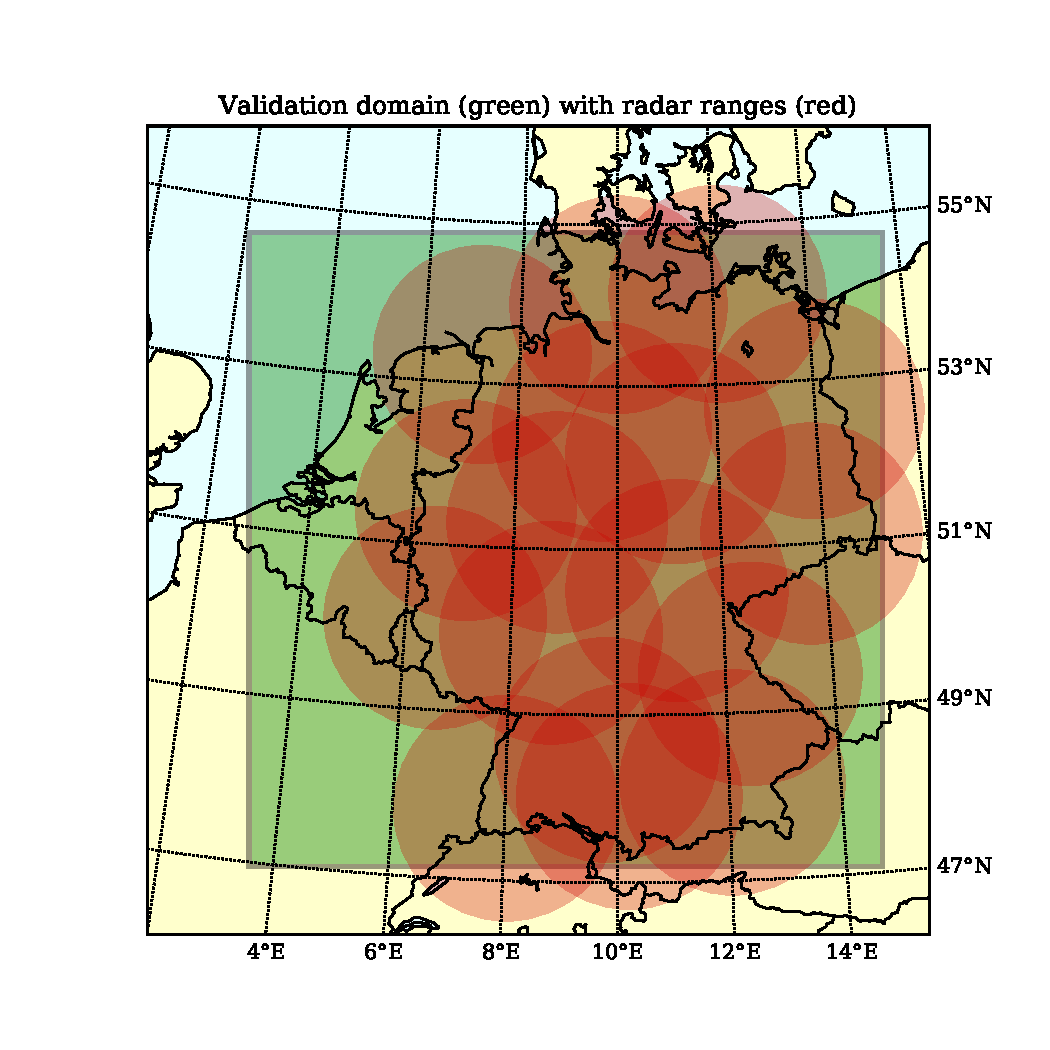
\includegraphics[width=\textwidth]{Grafiken/Abbildungen/radolan_domain.pdf}
\caption{Map of the validation domain (green) with the ranges of the weather radars of the German weather radar network (red). The validation domain is the standard domain of the German weather radar network as defined in \citet{RADOLANkurz2018} and it comprises an area of \SI{900 x 900}{\kilo\metre} covering Germany and parts of its neighbouring countries.}
\label{fig:radolan_domain}
\end{figure}
The validation of the NWC\,SAF CI product is conducted with weather radar data from the RADOLAN RX radar composite, which is used as ground truth for the purposes of our study. The RADOLAN RX radar composite is generated by Deutscher Wetterdienst from observations of the German weather radar network, and is available every five minutes with a spatial resolution of \SI{1 x 1}{\kilo\metre}.  It contains uncorrected radar reflectivity observations and is obtained from 17 C-band radars located throughout Germany with an approximate observing range of \SI{150}{km} each \citep{RADOLANkurz2018}. The domain spans \SI{900 x 900}{\kilo\metre} with a spatial grid resolution of \SI{1 x 1}{\kilo\metre}, and is considered as the validation region for our study. It is shown by the green shaded area in Fig. \ref{fig:radolan_domain}, and comprises Germany, large parts of northeast France, the Netherlands, Luxembourg, large parts of Belgium and smaller parts of Switzerland, Austria, Poland and the Czech Republic. However, the domain is not fully covered by observations, which are shown as red circles in Fig. \ref{fig:radolan_domain}. It also has to be noted that there are relatively frequent outages of individual radars, which affects the quality of the instantaneous products.

\section{Case days}
In the validation study of the NWC\,SAF CI product v2016 by \citet{Karagiannidis2016}, four case days have been considered to validate the product: 25\textsuperscript{th} May 2010, 28\textsuperscript{th} June 2010, 2\textsuperscript{nd} July 2010 and 3\textsuperscript{rd} July 2010. To ensure consistency, three of the four case days are used. As there was no convective development over Germany for 28\textsuperscript{th} June 2010, this day is not considered here. In order to extend the basis for validation, three additional case days were added: 23\textsuperscript{rd} May 2012, 18\textsuperscript{th} June 2013 and 20\textsuperscript{th} June 2013. A synoptic overview of the three additional case days is given below. For a synoptic description of the other three case days, please refer to \citet{Karagiannidis2016}.

\subsection{23\textsuperscript{rd} May 2012}
On 23\textsuperscript{rd} May 2012 large parts of Western and Central Europe are influenced by a pronounced high pressure ridge which extends from the Iberian peninsula until the Baltic Sea (Fig.~\ref{fig:synoptik_20120523}). Corresponding to the high pressure ridge in the middle troposphere a ground high pressure system is located over Scandinavia (Fig.~\ref{fig:synoptik_20120523}a). Over the eastern Atlantic ocean a quite distinct height trough expands from Iceland to the south with several corresponding low pressure systems at the ground. This large scale weather pattern leads to a north eastern flow towards Central Europe. 

Looking at the surface pressure chart (Fig.~\ref{fig:synoptik_20120523}b) it can be seen, that the pressure gradients are relatively low over Western and Central Europe but are stronger along the coasts of the Northern and Baltic Sea along the frontal zone. 

Concerning the GFS reanalysis charts for the KO index / vertical movement (Fig.~\ref{fig:synoptik_20120523}c) and LI/ CAPE (Fig.~\ref{fig:synoptik_20120523}d), it has to be noted that the atmospheric composition is quite unstable which can be seen from the strongly negative values of the KO index. Moreover there are large areas in Central Europe with strong vertical movement induced by the rather high temperatures of the day. Especially over Northern Germany the CAPE is moderately elevated and the LI shows high values, which both indicates a high potential for convective development.

\begin{figure}[htbp]
	\centering
	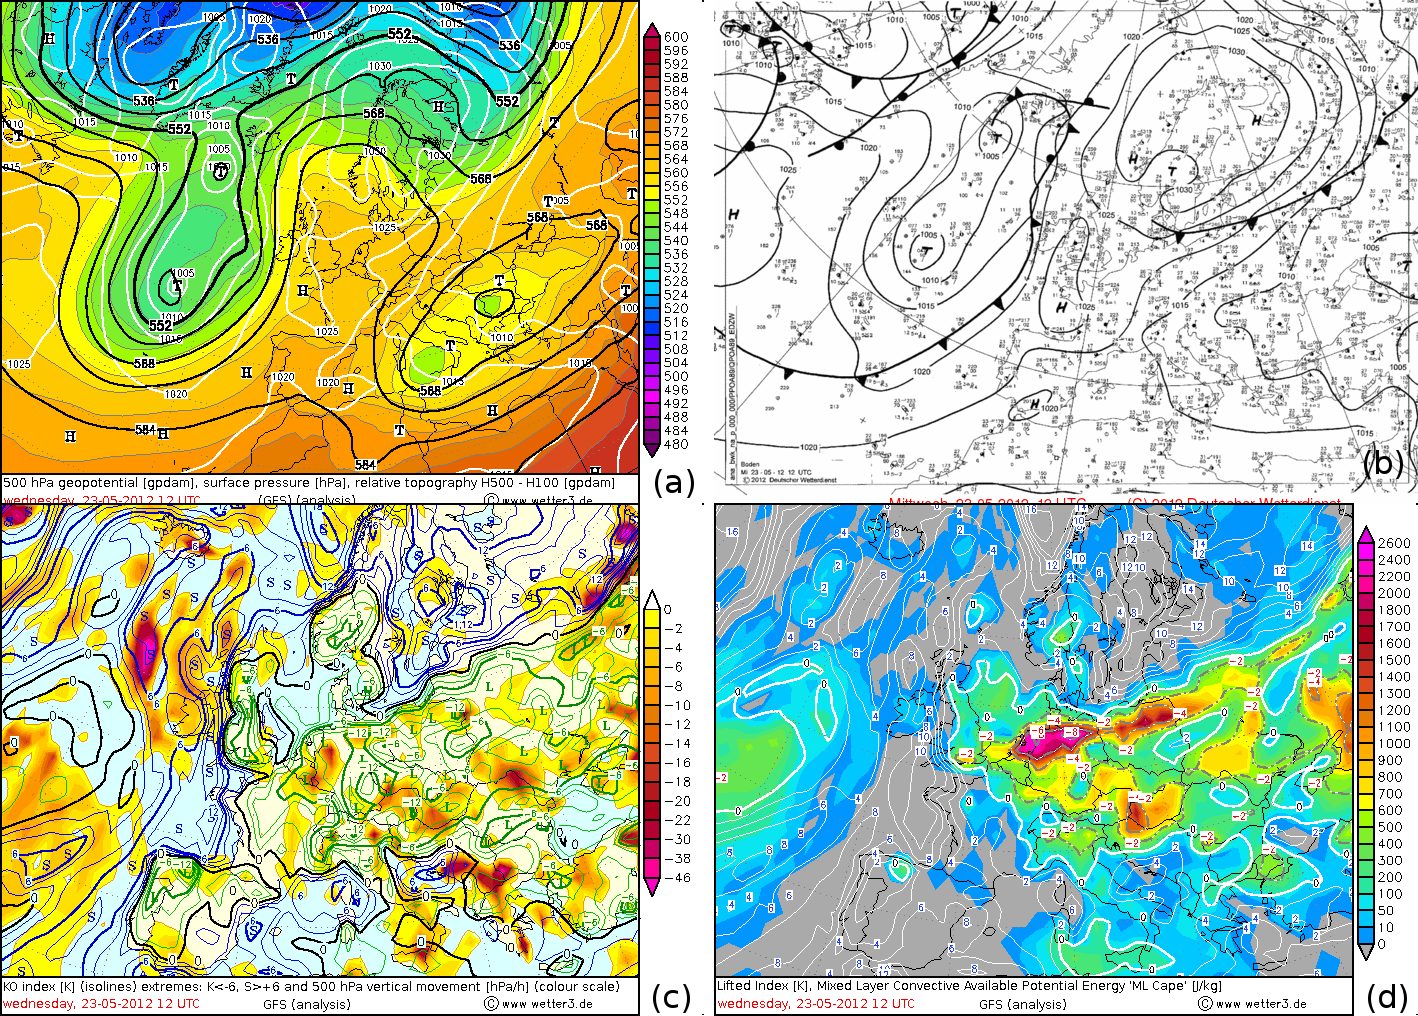
\includegraphics[width=0.8\linewidth]{Grafiken/Abbildungen/synoptik_20120523.png}
	\caption{Synoptic overview for 23\textsuperscript{rd} May 2012, 12:00 UTC, (a) \SI{500}{\hecto\pascal} geopotential, surface pressure and relative topography \SI{500}{\hecto\pascal} - \SI{1000}{\hecto\pascal}, source: www.wetter3.de, (b) Surface pressure analysis, source: Deutscher Wetterdienst, (c) KO index and \SI{500}{\hecto\pascal} vertical movement, source www.wetter3.de, (d) Lifted Index and Mixed Layer Convective Available Potential Energy, source: www.wetter3.de}
    \label{fig:synoptik_20120523}  
\end{figure}

\subsection{18\textsuperscript{th} June 2013}
On 18\textsuperscript{th} June 2013 the weather over Central Europe was dominated by a upper level high pressure ridge which extended from Northern Africa to South West and Central Europe while a upper level trough expanded from Iceland south to the Iberian peninsula where a higher level low pressure core was situated (Fig.~ \ref{fig:synoptik_20130618}a). This large scale weather pattern lead to a southern flow to Central Europe. Along the frontal zone of the upper level low pressure system, hot and unstable air masses where transported northwards leading to an unstable atmospheric composition and a pronounced heat wave over south western Central Europe.

In the ground pressure field several smaller low pressure systems are located below the upper level high pressure ridge, also leading to an unstable atmospheric composition (Fig.~\ref{fig:synoptik_20130618}]b). 

The KO index / vertical movement chart (Fig.~\ref{fig:synoptik_20130618}c) shows strong vertical movements over South West and Central Europe while the KO index is only slightly negative, indicating only a slightly unstable atmosphere. The LI / CAPE chart (Fig.~\ref{fig:synoptik_20130618}d) shows, that strongly elevated CAPE and also strongly negative LI values are present over Central Europe, indicating a strong potential for convective development.

\begin{figure}[htbp]
	\centering
	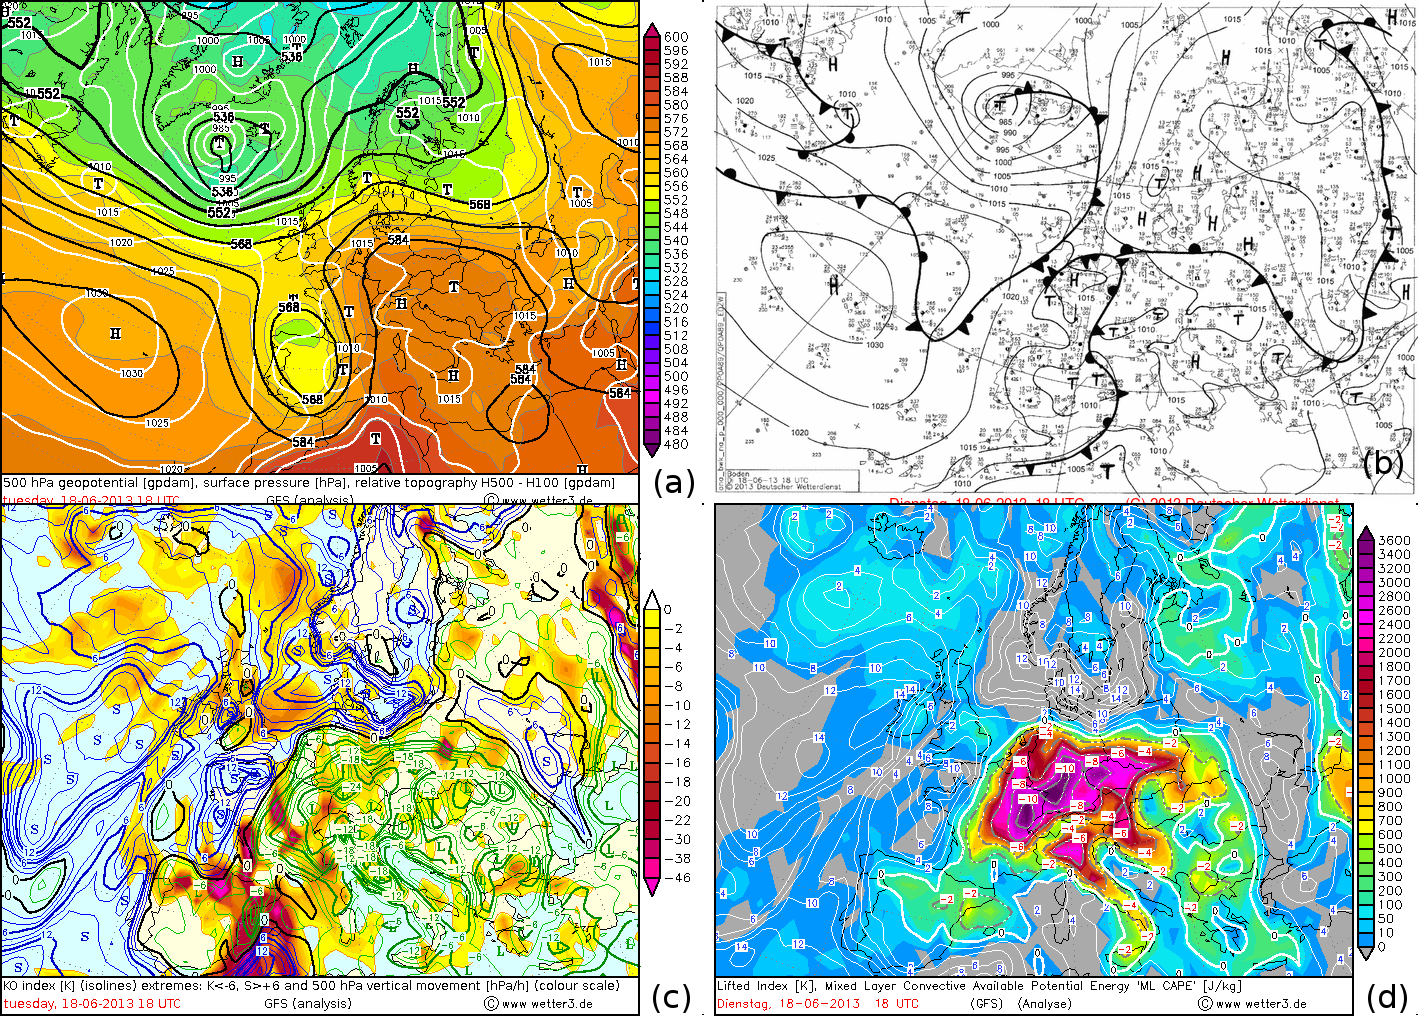
\includegraphics[width=0.8\linewidth]{Grafiken/Abbildungen/synoptik_20130618.png}
	\caption{Same as Fig.~\ref{fig:synoptik_20120523} but for 18\textsuperscript{th} June 2013, 12:00 UTC}
    \label{fig:synoptik_20130618}  
\end{figure}


\subsection{20\textsuperscript{th} June 2013}
The weather situation of the 20\textsuperscript{th} June 2013 was quite similar to the one on 18\textsuperscript{th} June 2013. The large scale weather pattern is similar but the higher level low pressure core situated over Southern France gained more influence on the weather in Central Europe (Fig.~\ref{fig:synoptik_20130620}a). Additionally a heat low pressure system formed in the hot air over North Eastern Germany with a convergence line on its western boundary as can be seen in the ground pressure field (Fig.~\ref{fig:synoptik_20130620}b). Along this convergence line several thunderstorms formed and in the evening the cold front of the low pressure system over Southern France reached Germany leading to the formation an organised thunderstorm line.

The KO index / vertical movement chart (Fig.~\ref{fig:synoptik_20130620}c) shows strong vertical movements over North West Germany and also a strongly negative KO index over this area, indicating a quite unstable atmosphere. The LI / CAPE chart (Fig.~\ref{fig:synoptik_20130620}d) shows, that strongly elevated CAPE and also strongly negative LI values are present over the most parts of Germany, indicating a strong potential for convective development.

\begin{figure}[htbp]
	\centering
	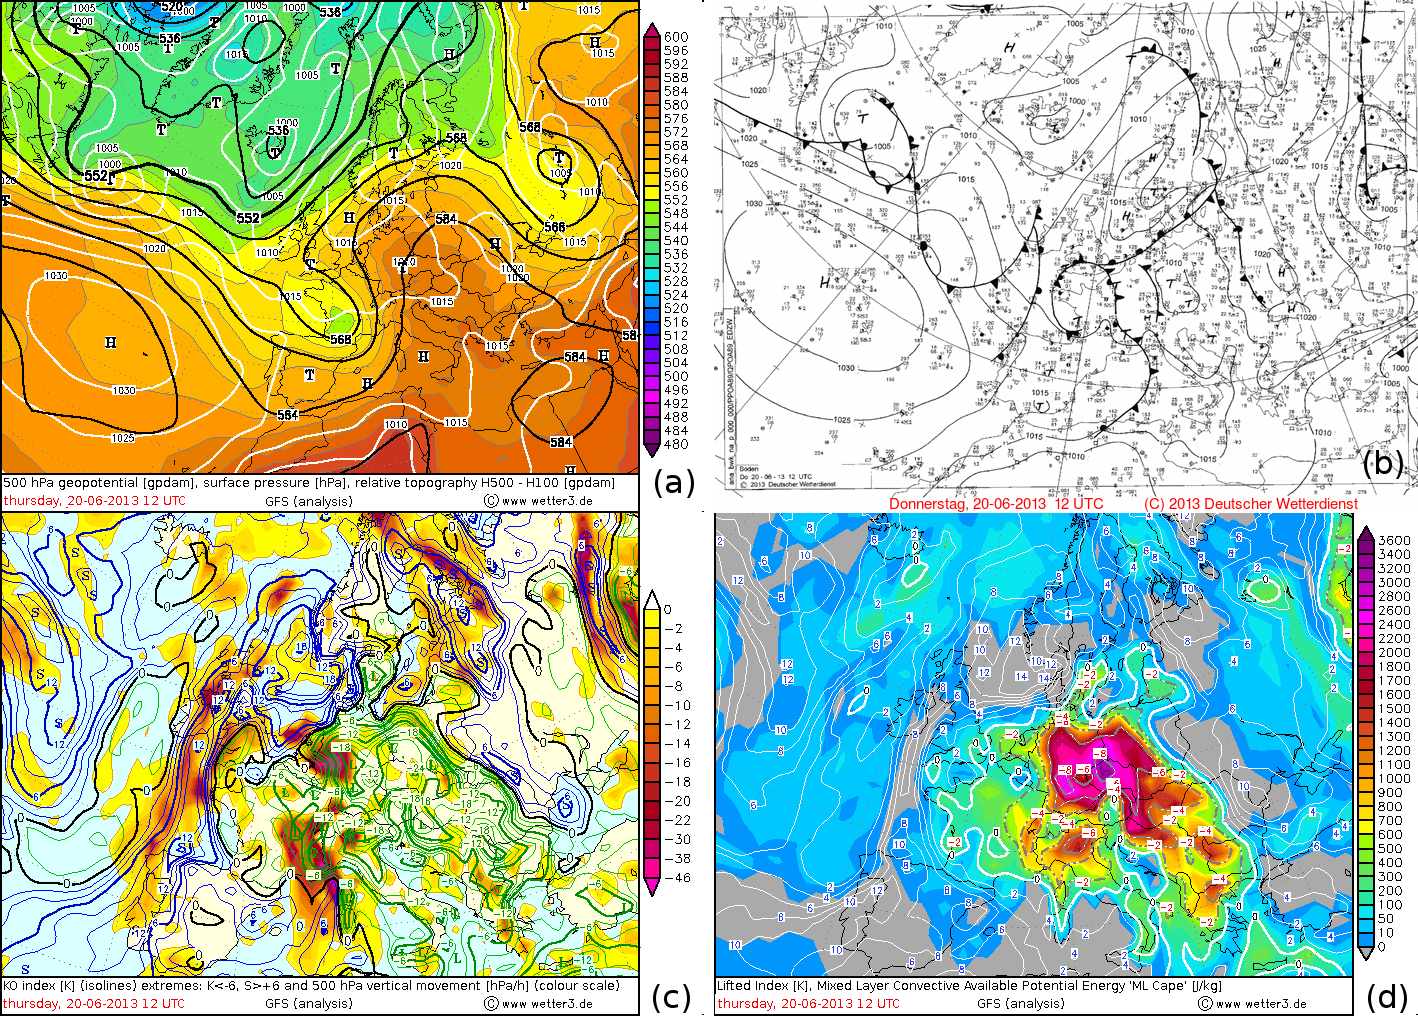
\includegraphics[width=0.8\linewidth]{Grafiken/Abbildungen/synoptik_20130620.png}
	\caption{Same as Fig.~\ref{fig:synoptik_20120523} but for 20\textsuperscript{th} June 2013, 12:00 UTC}
    \label{fig:synoptik_20130620}  
\end{figure}
\chapter{Methods}
In the present chapter, the general methodology and approach chosen for the validation of the NWCSAF CI product is presented.

\section{Validation region and parallax correction}
The validation region of this study is defined by the standard domain of the German weather radar network as given in \citet{RADOLANkurz2018}, which spans \SI{900 x 900}{\kilo\metre} with a spatial resolution of \SI{1 x 1}{\kilo\metre}. All satellite observations and products have been interpolated to this grid using nearest neighbour interpolation.

The slanted viewing angle of Meteosat SEVIRI for Central Europe causes an apparent shift of cloud fields in the satellite imagery. This shift depends on the cloud-top height and is mainly in northward direction for our viewing geometry. The effect is called "parallax effect" and typically leads a mismatch between radar-derived convective precipitation data (which do not suffer from such a shift) and the satellite imagery. If we look at combined cloud-precipitation-structures at the kilometer-scale, the parallax shift is of similar magnitude and  can not be ignored. Hence, a geometric transformation of the satellite fields has to be applied to correct for this effect.

As mentioned above, Meteosat SEVIRI data and NWCSAF products have been reprojected onto the radar grid with an approximative grid spacing of one kilometer. This fine grid ensures that no information from satellite observations is lost in the data combination. Now, the task of the parallax transform is to reproject the satellite data in such a way that cloud fields and structures appear like being sensed from a (hypothetical) nadir viewing platform. This ideal transformation is however hard to achieve because of several issues:
\begin{itemize}
\item \textbf{semi-transparency of multi-layer problem:} For semi-transparent or multi-layer clouds it is hard to assess where directly radiation comes from. That might also differ from channel to channel and not enough information is in the satellite data to reconstruct the cloud field three-dimensionally and independently apply shifts of separate layers.
\item \textbf{spatial resolution problem:} Cloud-top height estimates are needed for parallax correction. These are typically derived from narrow-band, but "coarse" resolution infrared channels. For some of the applied cloud-top height methods, the spatial resolution is even coarser than the standard Meteosat pixel resolution. Therefore, it can not be expected that the cloud texture information is meaningfully contained in the cloud-top height product. 
\item \textbf{information loss:} An ideal parallax correction would remove information obtained from the cloud-side observation. This information would be lost and holes in the images would appear behind the cloud towers where no remote sensing signal is available.
\end{itemize}
With these issues in mind, we choose the following strategy for applying a parallax transform:
\begin{enumerate}
\item Cloud-top height products have been calculated. For simplicity, we chose the TROPOS cloud product production chain that is based on NWCSAF version 2013 using ECMWF forecasts as numerical simulation.
\item Cloud-top height products have been smoothed. The reason for the smoothing choice is that sharp edges in the cloud-top height product destroy the texture of the parallax-corrected satellite images and introduces unwanted artifacts into the results. We choose a sequence of two filters: first a percentile filter based on the 90-th percentile with a footprint of 21 km, second a convolution filter with a Gaussian kernel of 9 km width.
\item Parallax-corrected latitude and longitude positions of clouds have been calculated based on the source code provided by the NWCSAF team.
\item The new lat-lon positions define a distortion of the original grid. We use a readily available image warping algorithm which utilizes cubic interpolation to remap the distorted grid onto the radar grid (the skimage.transform.warp function provided by the Scikit-Image Python library)  
\end{enumerate}

\begin{figure}[!b]
\centering
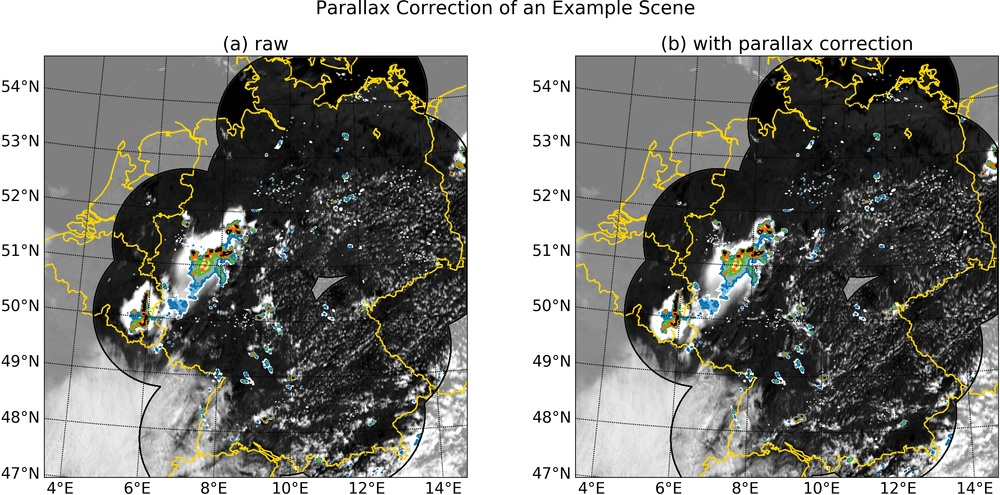
\includegraphics[width=\textwidth]{Grafiken/Abbildungen/parallax_example.jpg}
\caption{An example scene for a combination of Meteosat SEVIRI HRV reflectances (gray shades) and Radolan RX radar reflectivities (colored shades) for 23 May 2012, 12:30 UTC . (a) Raw combination of regridded data and (b) combination of data with HRV reflectance being parallax corrected. Coastline and country borders are in yellow, region with no radar coverage has been masked out with gray overlays.}
\label{fig:parallax_example}
\end{figure}
An example of the parallax transform applied to the HRV reflectances is shown in Fig.~\ref{fig:parallax_example}. The image transformation significantly improves the overlap between radar-derived precipitation signatures and cloud features. Some distortion of the cloud fields is still visible, we however consider the result of the parallax transform method as a good compromise. 


\section{Definition of Ground Truth}
\label{sec:haci}
Using the RADOLAN RX composite, isolated convective objects have been identified using the method described in \citet{Haberlie_2015}. First the radar data (Fig.~\ref{fig:haberlie}a) has been masked using a reflectivity factor threshold of \SI{35}{\dbZ} (Fig.~\ref{fig:haberlie}b) to delineate convectively active regions. These regions are then grouped into objects by requiring connectivity. A buffer mask is generated around existing objects as well as the border of the radar range using a buffer radius of \SI{15}{\kilo\metre}. This buffer mask is applied to the next time step, in order to identify newly developing convective objects (Fig. \ref{fig:haberlie}c). Finally, all newly developed convective objects outside the buffer mask with a reflectivity factor of over \SI{35}{\dbZ} are considered as new convective objects, which have thus initiated within the last five minutes (Fig.~\ref{fig:haberlie}d). Requiring a minimum object life time of \SI{30}{\minute} together with some additional  criteria, only objects are retained which have a sufficient life time to be considered as convective objects (Fig.~\ref{fig:haberlie}e). Convective object identification is done at five minutes time resolution for all case days, and is subsequently aggregated to \SI{15}{\minute} time steps to match the temporal resolution of the NWC\,SAF CI product. These object represent the ground truth used further for the validation of the CI product.

\begin{figure}[htbp]
\centering
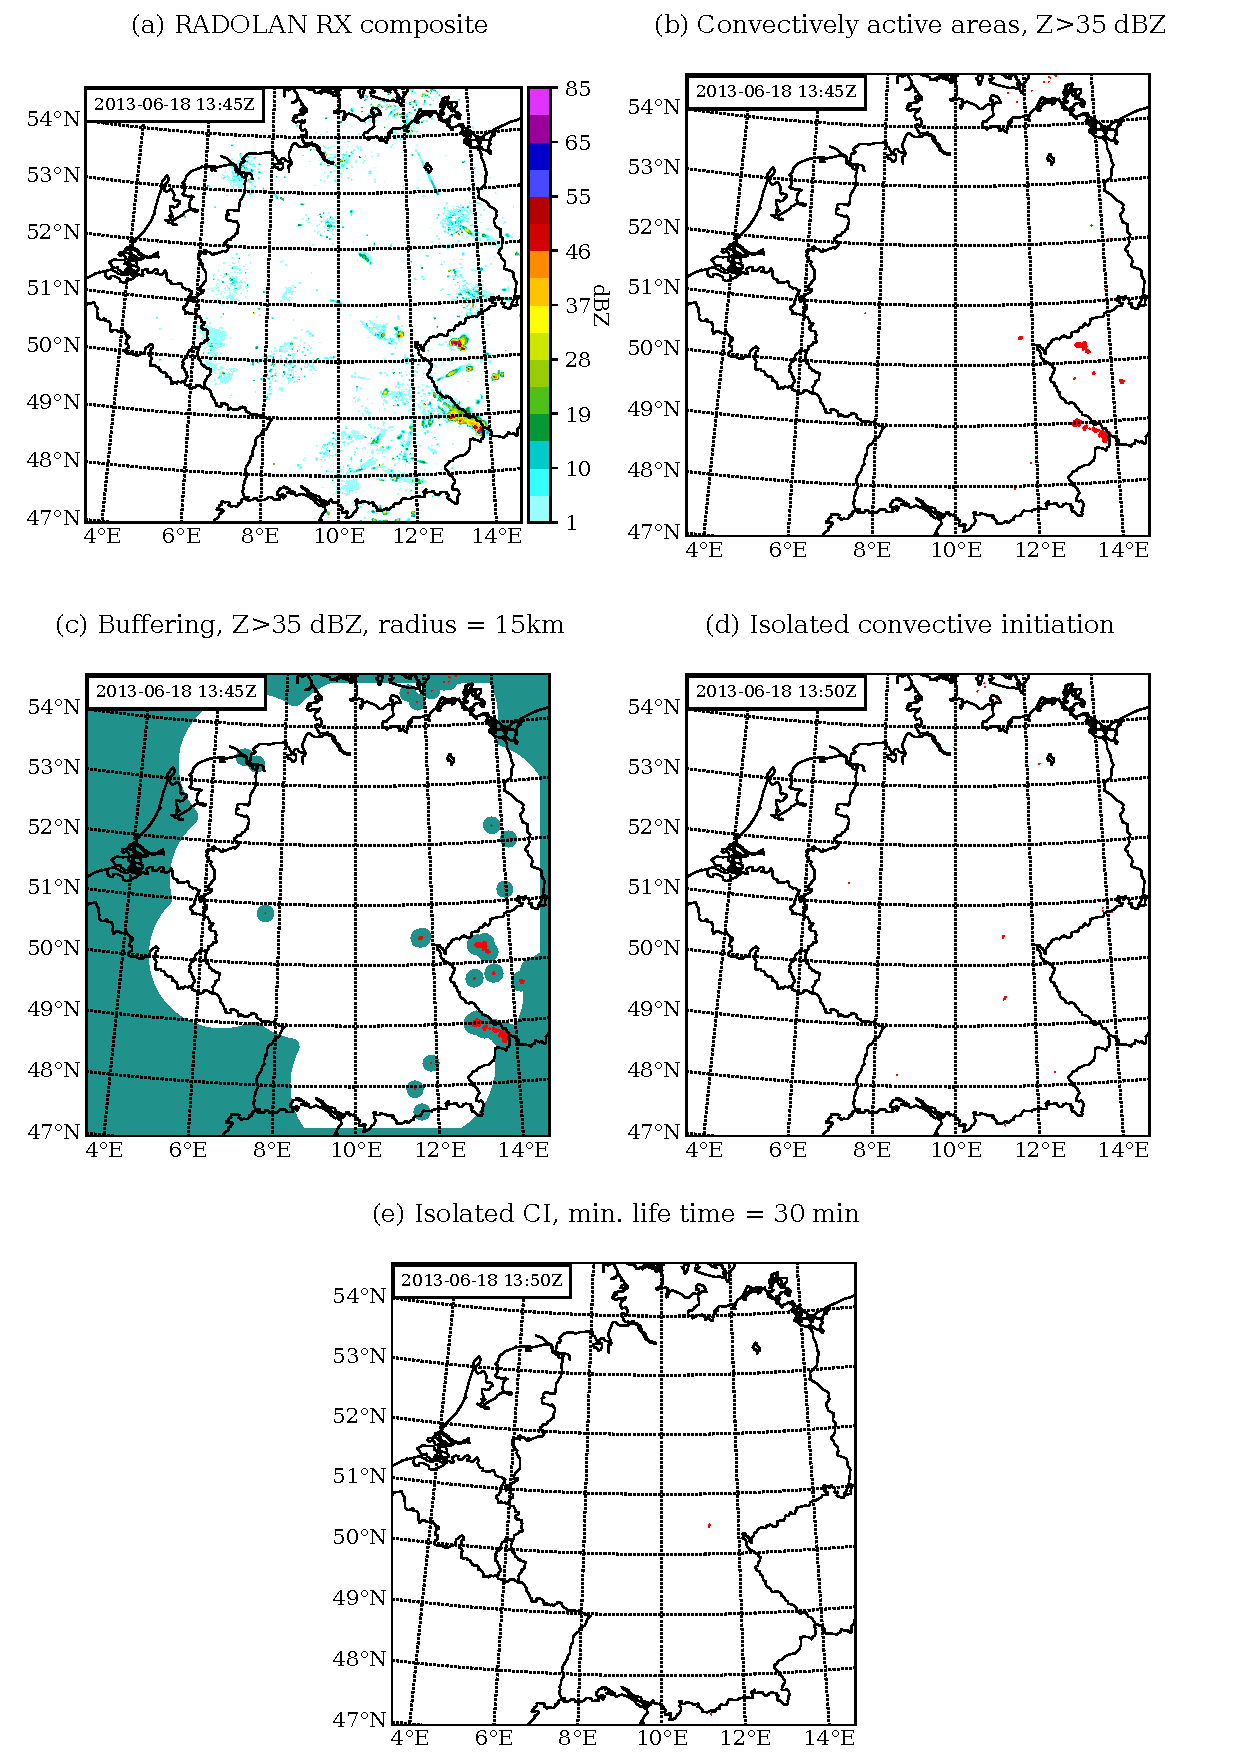
\includegraphics[height=\textheight]{Grafiken/Abbildungen/haberlie_prinzip.pdf}
\caption{Principle of deriving the ground truth. Using weather radar data (a), the data are masked using a reflectivity threshold of \SI{35}{\dbZ} to derive convectively active areas (b). Then these objects are buffered using a buffer radius of \SI{15}{\kilo\metre} (c). Using these buffers the, data of the next time step is masked, so that only isolated newly developing convection is taken into account (d). After that, to only consider precipitating objects with an adequate life  time, all objects with a minimum life time below \SI{30}{min} are masked out (e).}
\label{fig:haberlie}
\end{figure}

It has to be noted that this definition of ground truth is rather strict and quite different from the approach chosen by \citet{Karagiannidis2016}.  

\section{Derivation of motion fields}
The motion of cloud fields in the satellite observations was estimated using the implementation of the TV-L1 optical flow algorithm proposed by \citet{Zach2007}. The Python interface to the OpenCV library \citep{opencV_library} has been used here. The algorithm parameters selected here where optimised using the MPI Sintel test dataset \citep{Butler:ECCV:2012}, and are given in Tab. \ref{tab:oflow}. Motion fields have been calculated from Meteosat's IR \SI{10.8}{\micro\metre} and HRV channels considering \SI{15}{\minute} time steps. 
The TV-L1 optical flow approach differs from the cross correlation-based approach by MecikalskiBedka2006 to derive atmospheric motion vectors (AMV) by allowing discontinuities in the flow field, and tends to be more robust against noise than other techniques of motion tracking Perez2013.

\begin{table}[htb]
\caption{opencv parameters used for the estimation of the optical flow using the method proposed \citet{Zach2007}}
\begin{tabular}{llS} 
\toprule
parameter & description & {value}\\ 
\midrule 
$\epsilon$ & stopping criterion threshold used in the numerical scheme & \num{0.01}\\ 
$\gamma$ & coefficient for additional illumination variation term & 0.4\\ 
$\lambda$ & weight parameter for the data term, attachment parameter & 0.2\\ 
$\mu$ & kernel size of the median filter & 1\\ 
$\tau$ & time step of the numerical scheme & 0.25\\ 
$\theta$ & Weight parameter for (u - v)\textsuperscript{2}, tightness parameter & 0.8\\ 
$\mathrm{N}_\mathrm{inner}$ & number of inner iterations  used in the numerical scheme & 7\\ 
$\mathrm{N}_\mathrm{outer}$ & number of outer iterations  used in the numerical scheme & 40\\ 
$\mathrm{N}_\mathrm{scales}$ & number of scales used to create the pyramid of images & 5\\ 
$\mathrm{S}_\mathrm{scales}$ & steps between scales & 0.5\\
$\mathrm{N}_\mathrm{warp}$ & number of warpings per scale & 5\\ 
\addlinespace
\bottomrule
\end{tabular}
\label{tab:oflow}
\end{table}

\section{Cloud objects}
\label{sec:cloud}
To validate the detections of the NWC\,SAF CI product and the detections of the radar based approach presented above, cloud objects have been derived. 

The cloud objects are based on the NWC\,SAF cloud mask product and the MSG HRV channel, as its higher spatial resolution allows for a better separability of cloud objects than the standard MSG resolution. As the HRV channel is in the visible spectrum, and so there is no data for the night time, only a time frame of twelve hours centered around noon CET (05:00 am UTC to 05:00 pm UTC) has been chosen for the derivation of cloud objects. This time frame has the advantage that there is data for all case days and it also avoids the time around sunrise and sunset where atmospheric scattering effects make the data not usable for our objective.

For the derivation of meaningful cloud objects, the rather high HRV spatial resolution also has the drawback that often very small non-convective clouds are derived as cloud objects leading to an artificially high rate of missed detections. To overcome this, the HRV field (Fig.~\ref{fig:hrv_seg}a) was filtered using a Gaussian filter (Fig.~\ref{fig:hrv_seg}b) and the objects were derived from the smoothed HRV field (Fig.~\ref{fig:hrv_seg}c and d). Additionally a minimum size an object has to have to be considered was set. To find suitable filter, minimum size and threshold parameters, a number of different parameters combination has been tested against the overlap size of ground truth objects and cloud objects for the 25\textsuperscript{th} May 2010. The result of the analysis is shown in Fig. \ref{fig:filter-parameters}. It turns out, that the two parameters with the highest impact on the overlap size are the size of the Gaussian kernel and the threshold used to define which parts of the HRV channel field are objects. The minimum size of the objects and the connectivity used to segment the objects does not seem to have a large influence. The maximum intersection size between ground truth and cloud objects can be achieved by a rather strong smoothing, setting the Gaussian filter parameter \textsigma~to 3, and setting the HRV threshold to \num{0.3}. Additionally, for the derivation of the cloud objects, to avoid too small objects, the minimum object size was set to \num{10} \SI{1x1}{\kilo\metre} pixels and the connectivity type to \num{8} neighbours. 
 
\begin{figure}[htbp]
\centering
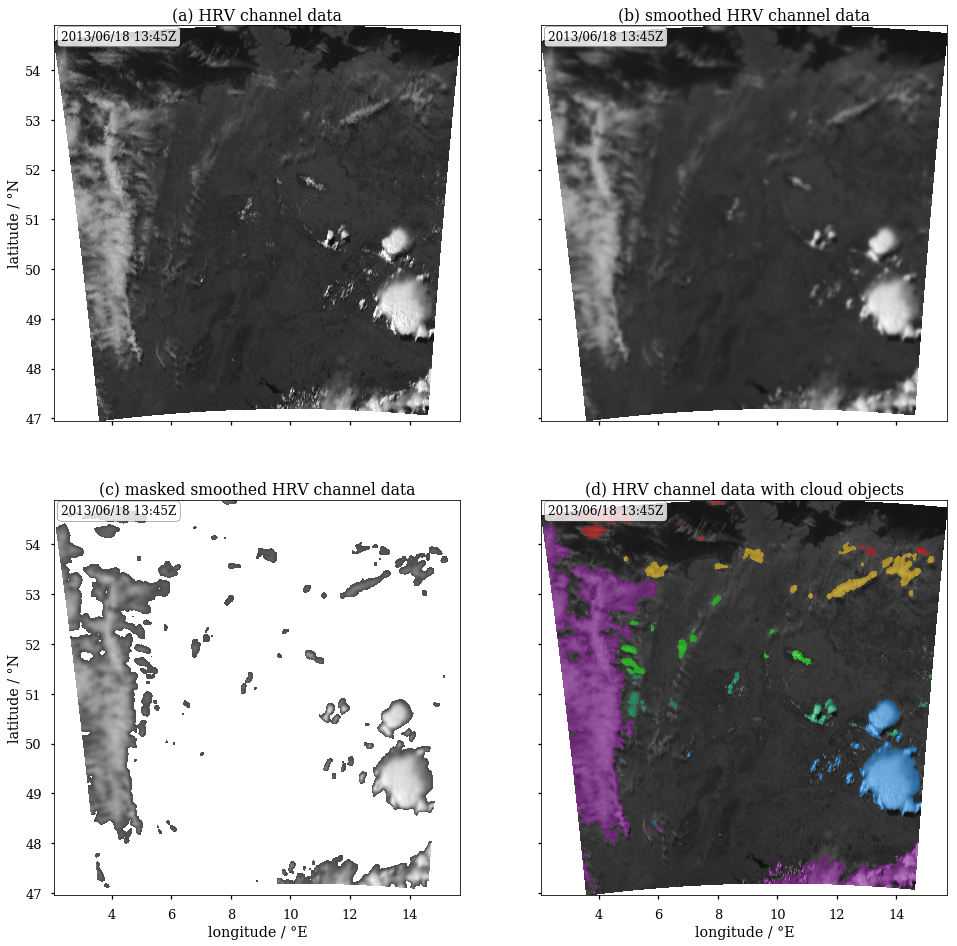
\includegraphics[width=\textwidth]{Grafiken/Abbildungen/wolkenobjektprinzip.png}
\caption{Principle of deriving the cloud objects. Using HRV channel data (a), the data are smoothed using a Gaussian blur filter with a \textsigma~value of 3 (b). Then these objects are buffered using a buffer radius of \SI{15}{\kilo\metre} (c). Using these buffers, the, data of the next time step is masked, so that only isolated newly developing convection is taken into account (d). }
\label{fig:hrv_seg}
\end{figure}

\begin{figure}[htbp]
\centering
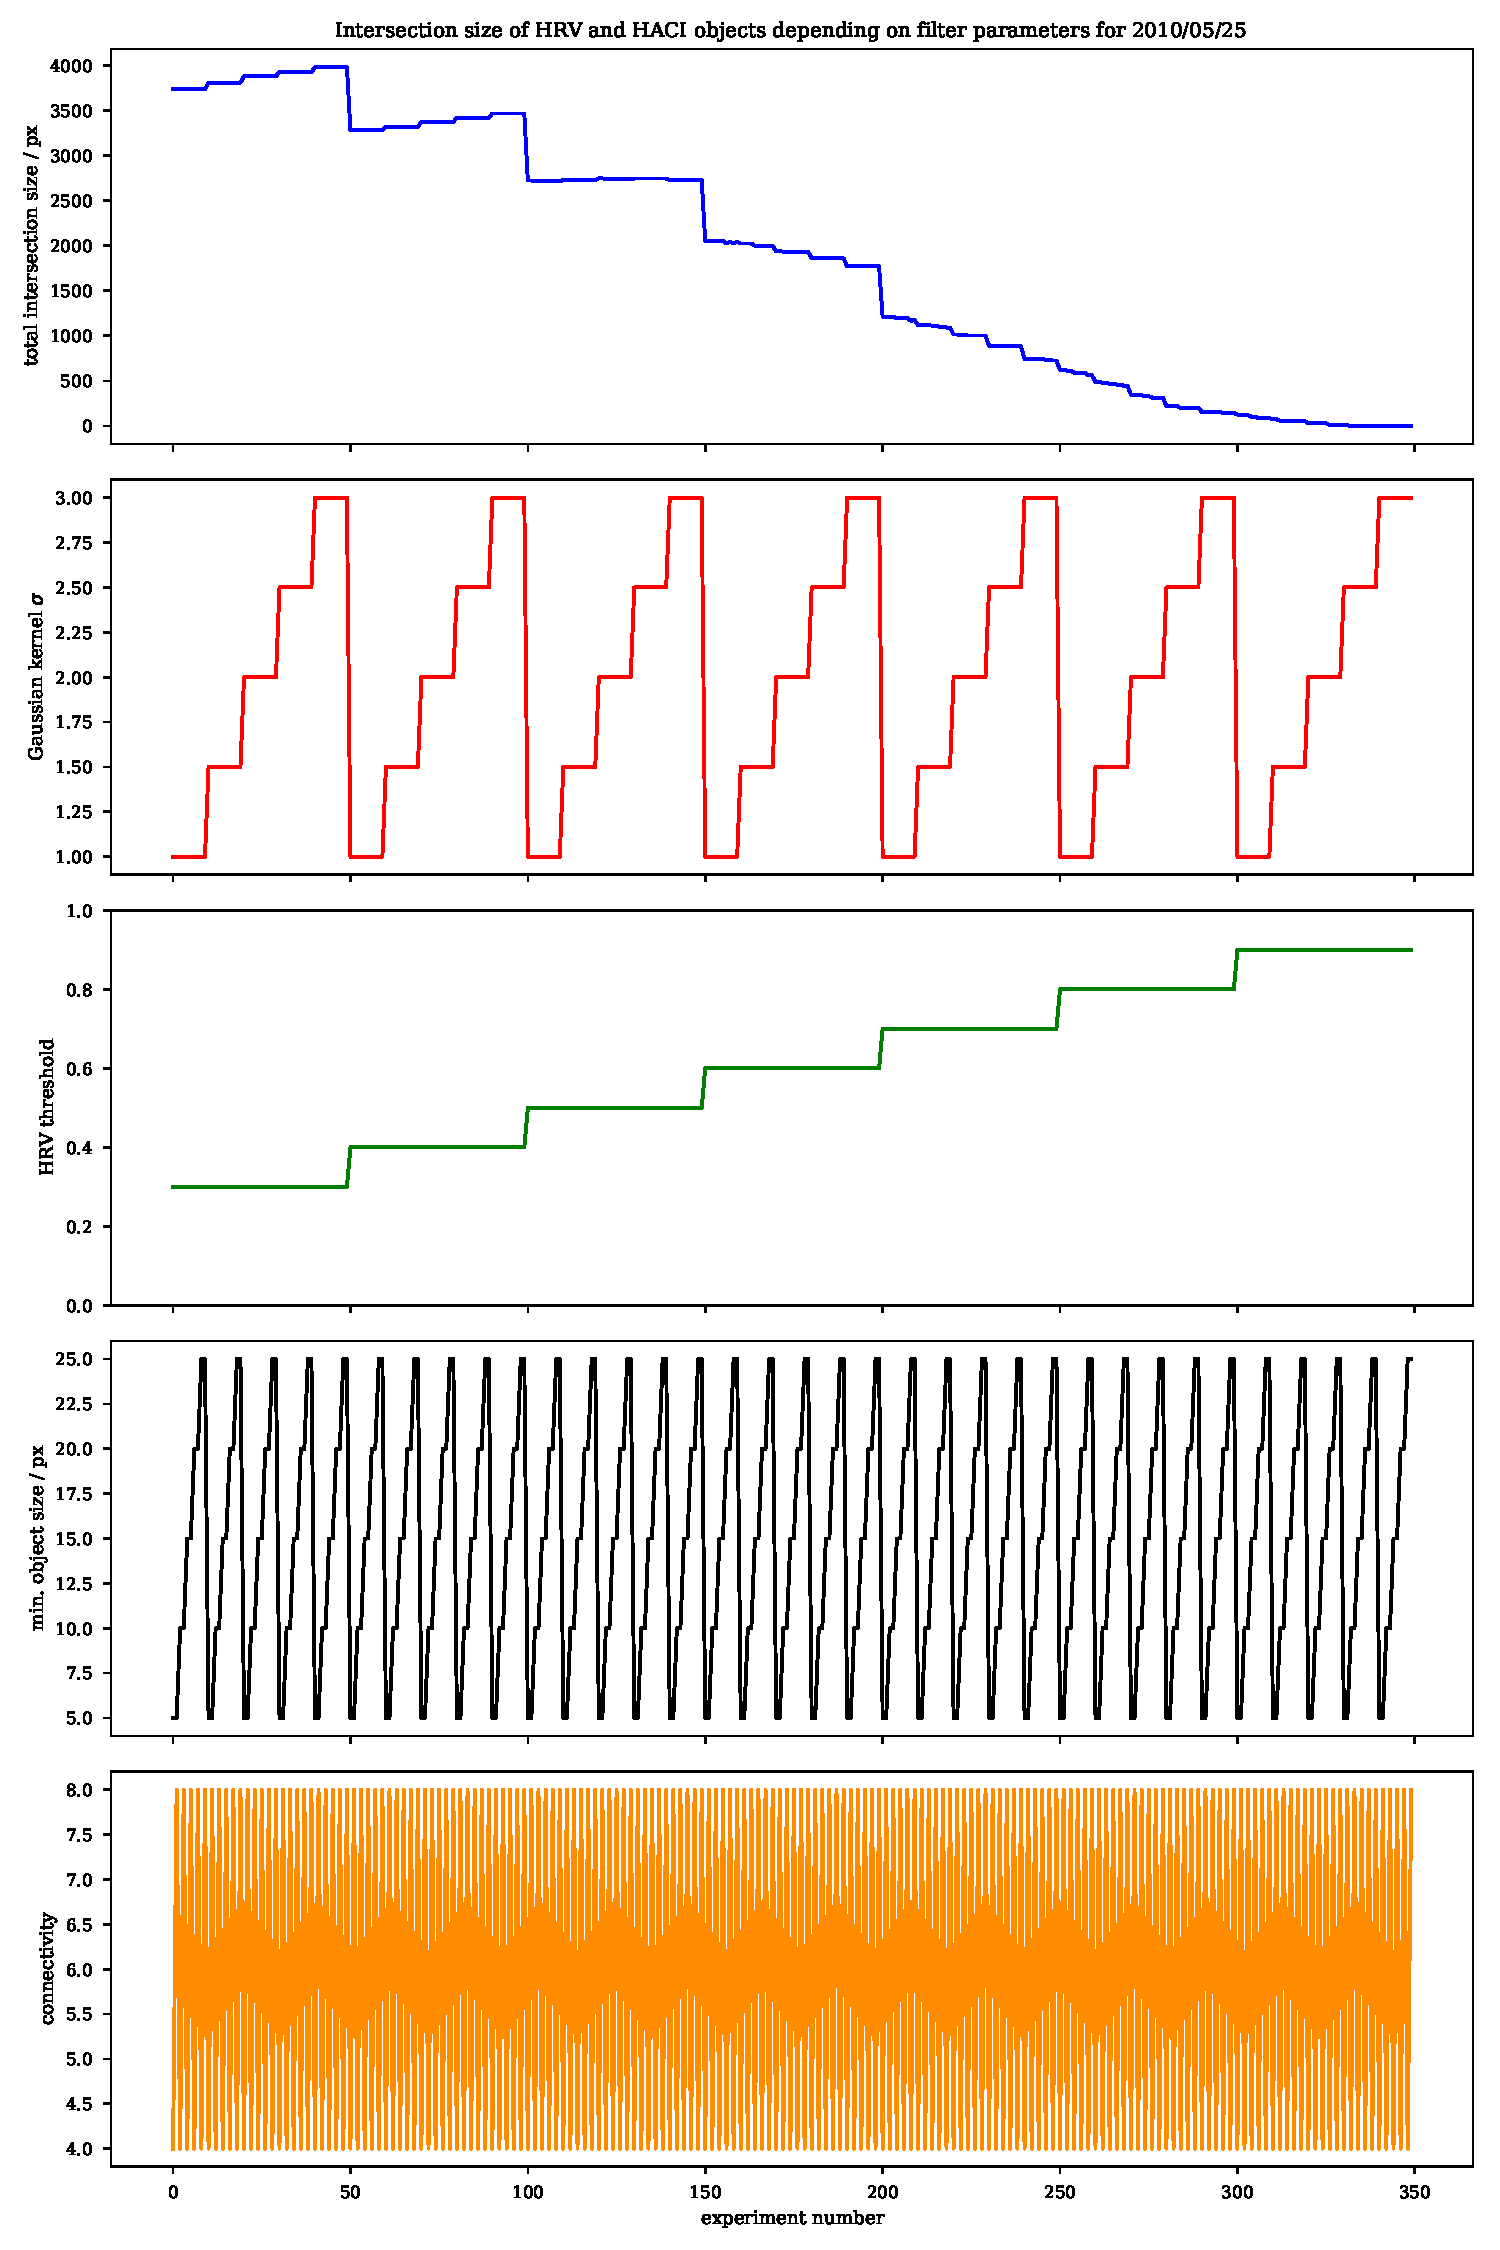
\includegraphics[height=\textheight]{Grafiken/Abbildungen/parameter_plot.pdf}
\caption{Intersection size (top most figure) between cloud and ground truth objects for combinations of four filters and segmentation parameters (figures below).}
\label{fig:filter-parameters}
\end{figure}

Objects tracks are created using the motion fields derived from the MSG HRV channel applying an overlap tracking approach. Starting from the first emergence of the particular object, the object is moved forward in time using the motion field. If the objects of the first and second time step overlap, an object path is created for the two time steps and so on. As the object structure often is quite complex with many splits and merges, mathematical graphs have been created to allow for an analysis of the object structure. Using the graphs, only single cell objects the part of the object tracks prior to splits and merges have been used in the further analysis. To allow for a comparison with the radar data, the tracks also have been parallax corrected using the cloud top height of the NWC\,SAF cloud height product.

To be consistent with the ground truth definition, only objects with a minimum life time of \SI{30}{\minute} have been considered in the further analysis.

\section{Validation approach}
\label{sec:validation}
The validation of the NWC\,SAF CI product  is based on cloud objects derived from MSG HRV data and weather radar detections as ground truth.

As shown in Fig. \ref{fig:schema}, the validation strategy is based on the intersection of cloud objects, detectrions by the CI product and ground truth objects. Given a track of a cloud object the cloud object is considered to be detected by the NWC\,SAF CI product if there is an intersection between the cloud object and pixels with a CI probability of strictly larger than \SI{0}{\percent}. If there is an intersection between the cloud object and pixels with different CI probabilities for one time step, only the highest CI probability is counted, and if there are more than one intersections of the cloud object and CI pixels along the object track, only the first intersection time step is counted. 

In the next step, starting from the CI detection time step, it is checked if there is an intersection between the cloud object and a ground truth object within the next \SI{30}{\minute}. If necessary, the track is getting extended by propagating the last available track point forward in time using the motion fields. If an intersection between a detected cloud object and a ground truth object can be observed within the next \SI{30}{\minute} it is counted as a true positive case for the highest CI probability level of the detection time step. If not, than it is counted as a false positive case.

If there are intersections with at least one ground truth object along the cloud object track and there are no intersections with CI pixels or the intersection with the first intersection with a ground truth object is earlier than the first intersection with CI pixels, the case is counted as false negative.

If a cloud object neither intersects with CI pixels nor with a ground truth objects it is counted as true negative.

The validation is performed separately for all CI levels. The confusion matrix of the validation approach is given in Tab.~\ref{tab:confusion}.

\begin{figure}[htbp]
\centering
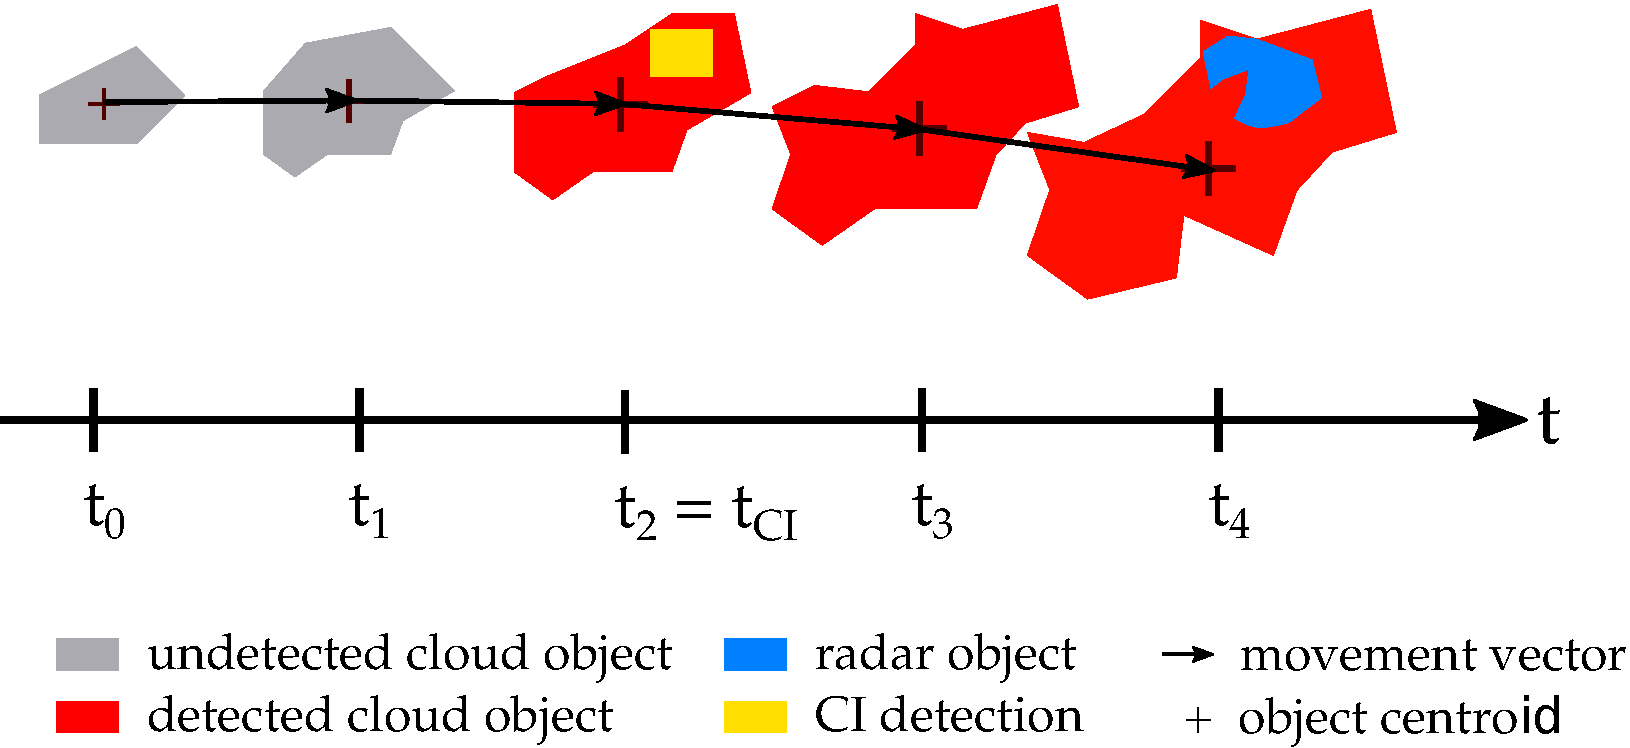
\includegraphics[width=0.9\textwidth]{Grafiken/Abbildungen/verification_scheme_new.pdf}
\caption{Schematic of the validation approach. Starting from a cloud object (grey and red) a cloud object track is created (denoted by the vector arrows) . If a CI object (yellow) is inside the validation area a new object track with validation region is created. If a radar object (blue) is detected inside the new \SI{30}{\minute} validation area the cloud object is counted as a true positive}
\label{fig:schema}
\end{figure}

\begin{table}[htbp]
\centering
\caption{Confusion matrix for the validation, TP = true positive, FP = false positive, FN = false negative, TN = true negative}
\begin{tabular}{cccc} 
\toprule
{CI product detection} & \multicolumn{2}{c}{weather radar detection} \\
					   \cmidrule{2-3}
					   & yes  & no \\
\midrule
yes                    &  TP  & FP \\
no                     &  FN  & TN \\ 
\addlinespace
\bottomrule
\end{tabular}
\label{tab:confusion}
\end{table}

For the assessment of the validation, several metrics can be derived from the confusion matrix. In this study the following are used:

\begin{itemize}
\item Probability Of Detection $\mathrm{POD} = \frac{\mathrm{TP}}{\mathrm{TP} + \mathrm{FN}}$, which is the probability to detect an event
\item False Alarm Ratio $ \mathrm{FAR} = \frac{\mathrm{FP}}{(\mathrm{FP} + \mathrm{TP})} $, which is a measure for the fraction of forecast that do not become events
\item Heidke Skill Score \citep{Heidke1926} $\mathrm{HSS} = \frac{2 (\mathrm{TP} \cdot \mathrm{TN}) - \mathrm{FP} \cdot \mathrm{FN}}{ (\mathrm{TP} + \mathrm{TF}) (\mathrm{FN} + \mathrm{TN}) (\mathrm{FP} + \mathrm{TN})}$, which is a measure of how good is the algorithm performance against a detection by chance
\item Critical Sucess Index $ \mathrm{CSI} = \frac{\mathrm{TP}}{\mathrm{TP} + \mathrm{FN} + \mathrm{FP}}$, which is a measure of how well forecasts events correspond to observed events 
\end{itemize}
\chapter{Pixel-based Analysis}

\section{Diurnal cycles}
\label{sec:diurnal_cycle}
In the following, we consider the total fraction of pixels that satisfy certain conditions. This fraction is also called coverage in the following. Two different variables are analysed:
\begin{enumerate}
\item The CI product data have been masked under the condition that each CI pixel is greater than or equal to a certain, selected CI threshold. This results in masks that select CI with probability equal to or greater than a certain value, e.g. all CI pixels are selected with a probability larger than 50\%, that combines the intervals 50-75\% and $>75$\%. In other words, the provided CI levels have been combined to cumulative CI probabilities for further analysis with the following meaning:
\begin{itemize}
    \item $\textrm{Prob}_{CI}\ge 0\%$  $\equiv$  CI indicator interval $]0, 100] \%$
    \item $\textrm{Prob}_{CI}\ge 25\%$  $\equiv$  CI indicator interval $]25, 100] \%$, etc.
\end{itemize}
\item Radar RX data are masked under the condition that radar reflectivities are greater than a threshold of 35 dBZ. The fractional coverage is called $f_{>35 \mathrm{dBZ}}$.
\end{enumerate}

The fractions of pixels that satisfy the conditions mentioned above are calculated for each time slot and date separately. The results are shown in Figs.~\ref{fig:dc20100523} to \ref{fig:dc20130620}. Looking at the diurnal cycle of the fractional coverage of low probability CI events (with $>0\%$ and $>25\%$), one can not recognise any reasonable connection to the diurnal cycle of higher probability CI events (with $>50\%$ and $>75\%$). The two low probability curves are in general very close together. Furthermore, there is more than one order of magnitude difference between the low and high probability CI counts. This means that the low probability CI categories are not well calibrated, and might be not reasonably connected to precipitation formation probability at all. Therefore, to our opinion, the low probability CI categories are likely to be useless.

In the next, we focus on the higher probability CI events (with $>50\%$ and $>75\%$). They cover only a very small fraction and therefore represent only a small number of events. Thus, conclusions based on the six case days are very likely to be statistically poorly significant. By inspection 
of Figs.~\ref{fig:dc20100523} to \ref{fig:dc20130620}, it can be seen that both categories show the main activity between noon and early evening. This is also the time period when the relative fraction of radar reflectivities $>35$ dBZ is increasing (except for the 28 June 2010 where no significant heavy precipitation was recorded) and where the temporal differences in $f_{>35\mathrm{dBZ}}$ are positive. This, of course, only gives a very general indication of an increased precipitation formation activity that comes along with an increase number of issued CI detections.

\begin{figure}
\centering
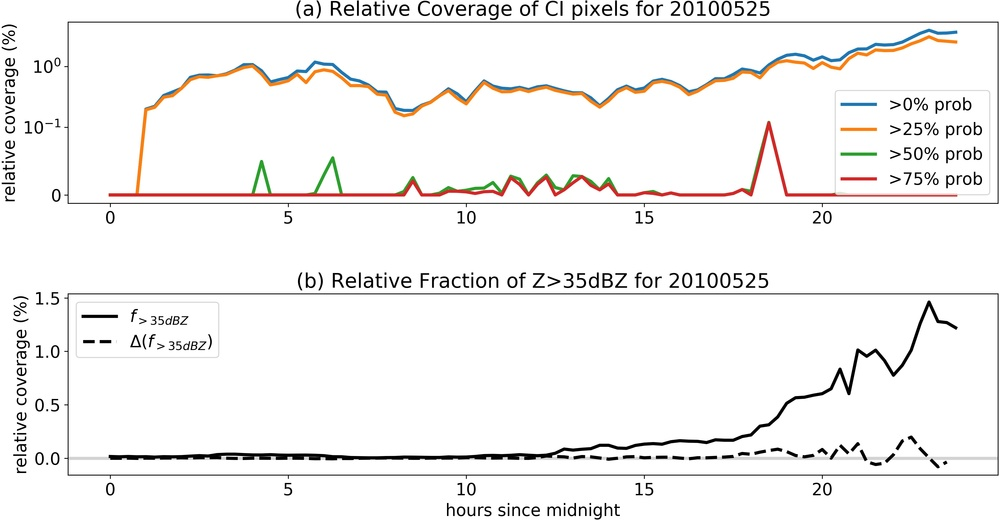
\includegraphics[width=\textwidth]{Grafiken/Abbildungen/diurnal_cycle_20100525.jpg}
\caption{Diurnal cycles of the fractional coverage of (a) CI pixels with a certain probability level (coloured lines) and (b) RX radar reflectivity pixels above 35 dBZ (black solid line) for the 25 May 2010. Please note that the upper part of the y-axis in panel a is logarithmic. The temporal change of $f_{>35\mathrm{dBZ}}$ is shown in panel b with a dashed black line. The curve has been smoothed with a running mean with a window of 3.}
\label{fig:dc20100523}
\end{figure}
%%%%%%%%%%%%%%%%%%%%%%%%%%%%%%%%%%%%%%%%%%%%%
\begin{figure}
\centering
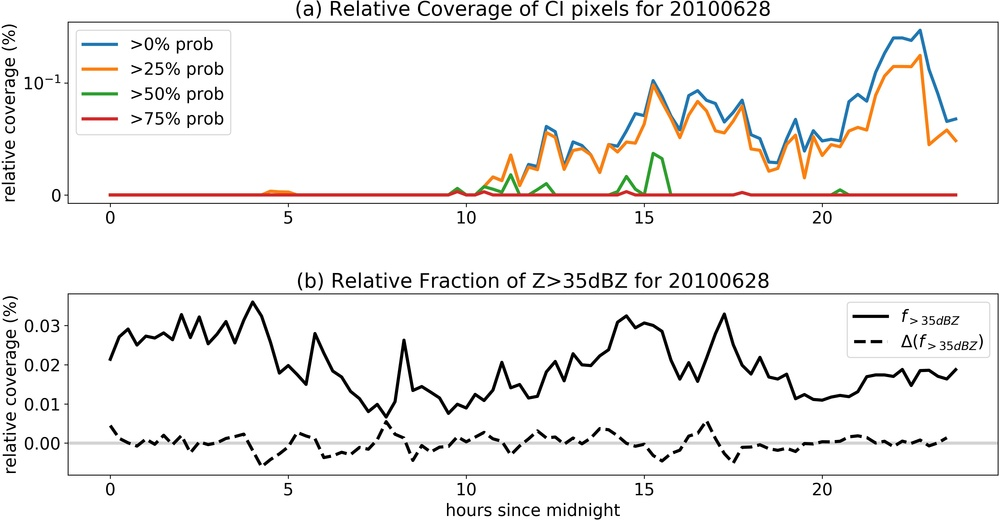
\includegraphics[width=\textwidth]{Grafiken/Abbildungen/diurnal_cycle_20100628.jpg}
\caption{Same as Fig.~\ref{fig:dc20100523}, but for the 28 June 2010.}
\label{fig:dc20100628}
\end{figure}
%%%%%%%%%%%%%%%%%%%%%%%%%%%%%%%%%%%%%%%%%%%%%
\begin{figure}
\centering
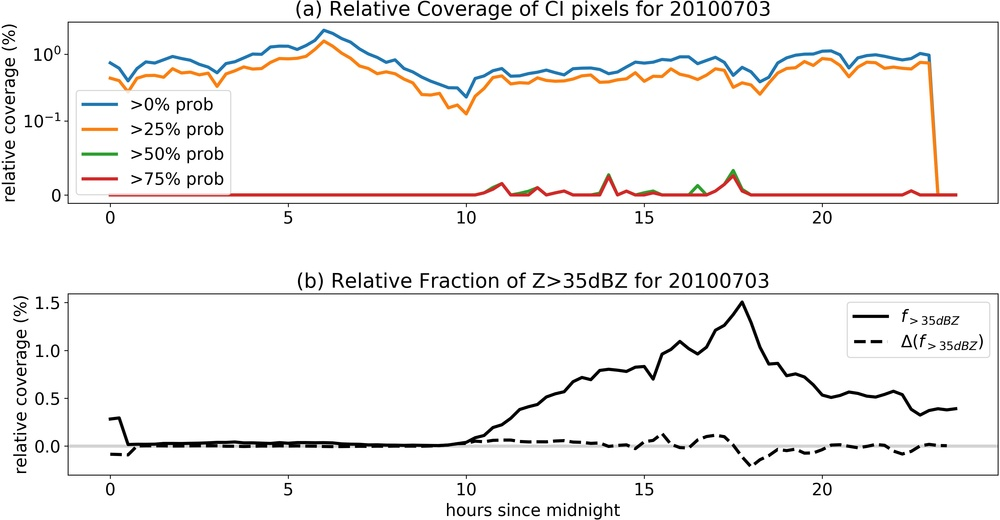
\includegraphics[width=\textwidth]{Grafiken/Abbildungen/diurnal_cycle_20100703.jpg}
\caption{Same as Fig.~\ref{fig:dc20100523}, but for the 3 July 2010.}
\label{fig:dc20100703}
\end{figure}
%%%%%%%%%%%%%%%%%%%%%%%%%%%%%%%%%%%%%%%%%%%%%
\begin{figure}
\centering
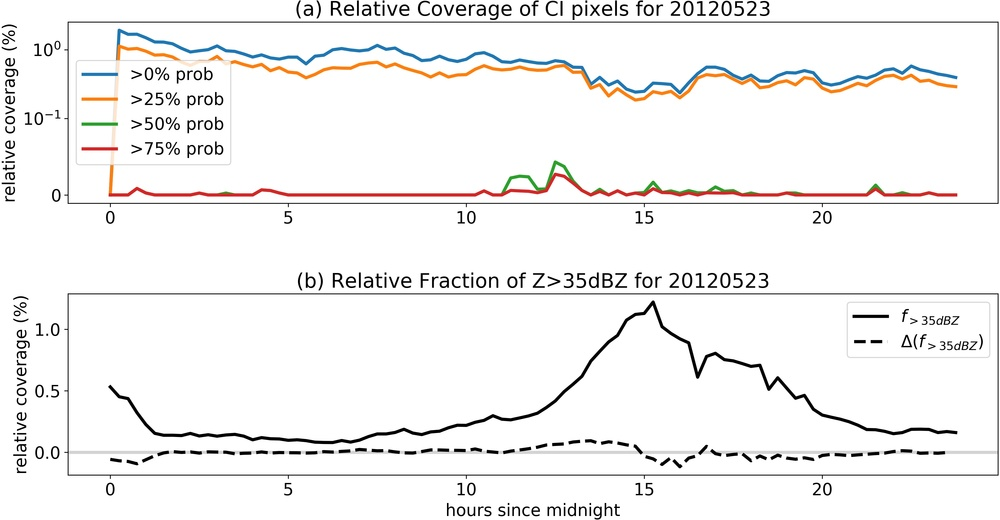
\includegraphics[width=\textwidth]{Grafiken/Abbildungen/diurnal_cycle_20120523.jpg}
\caption{Same as Fig.~\ref{fig:dc20100523}, but for the 23 May 2012.}
\label{fig:dc20120523}
\end{figure}
%%%%%%%%%%%%%%%%%%%%%%%%%%%%%%%%%%%%%%%%%%%%%
\begin{figure}
\centering
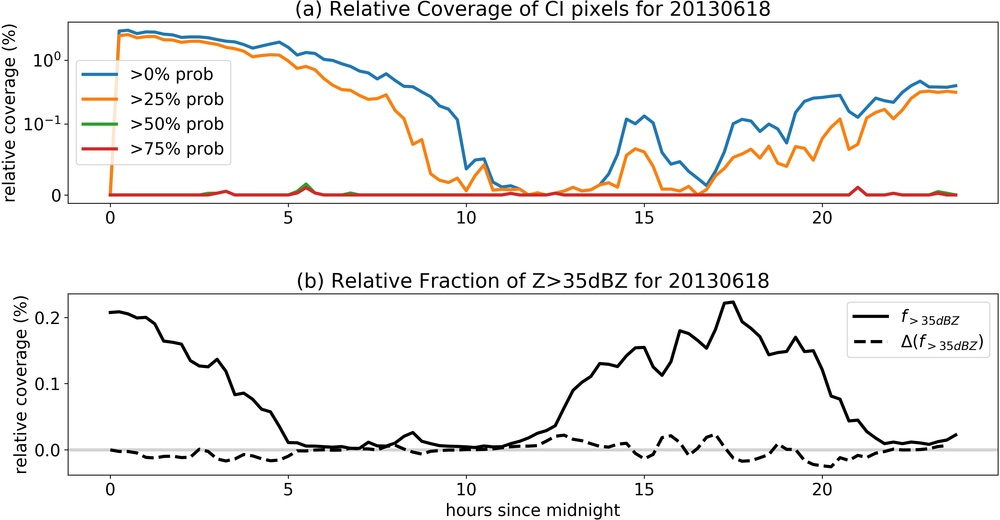
\includegraphics[width=\textwidth]{Grafiken/Abbildungen/diurnal_cycle_20130618.jpg}
\caption{Same as Fig.~\ref{fig:dc20100523}, but for the 18 June 2013.}
\label{fig:dc20130618}
\end{figure}
%%%%%%%%%%%%%%%%%%%%%%%%%%%%%%%%%%%%%%%%%%%%%
\begin{figure}
\centering
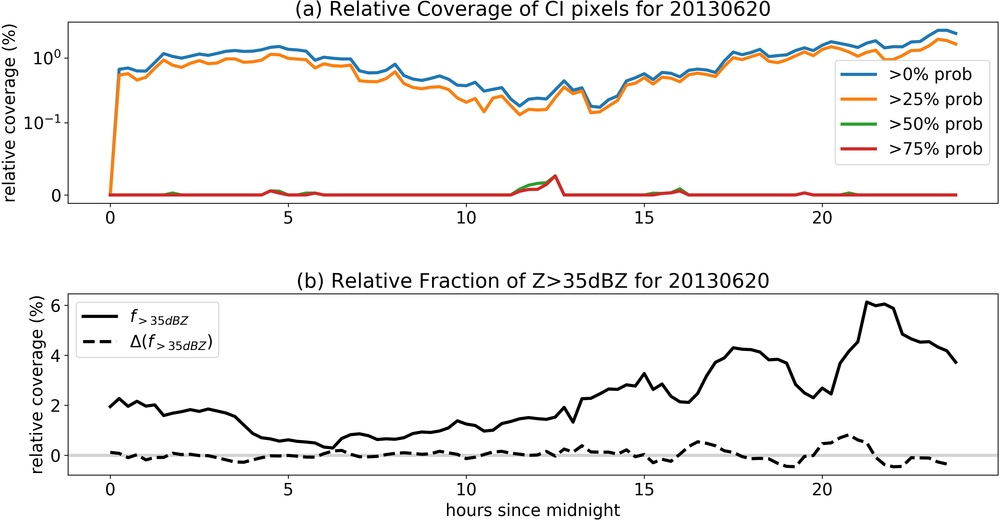
\includegraphics[width=\textwidth]{Grafiken/Abbildungen/diurnal_cycle_20130620.jpg}
\caption{Same as Fig.~\ref{fig:dc20100523}, but for the 20 June 2013.}
\label{fig:dc20130620}
\end{figure}

\section{Connection between CI detections and already existing precipitation}
From the movies \footnote{hosted at https://owncloud.gwdg.de/index.php/s/nwiyGQBFbN1FaH9, visited at 8 Nov 2018} generated by TROPOS for the case days which combine the CI product with radar data, one could get the impression that a significant fraction of CI detections occur in regions where radar reflectivities are already large. Depending on the interpretation of the CI product, a CI detection within or close to radar reflectivity contours $>35$ dBZ would be a false detection, as we would require that the CI detection marks a newly  developing precipitation cell and not an already existing one. In the above argument, we already used the word "cell". From a realistic precipitation field, it is often not clear what a "cell" is and how newly formed precipitation can be objectively detected. 

As noted above, the fraction of low probability CI detections is not connected to their higher probability counterpart and also does not follow the diurnal cycle in heavy precipitation changes. It is indeed the low probability CI field that has significant overlap with high radar reflectivities (not shown) and which introduces this above mentioned impression when viewing the movies. 

In contrast, the higher probability CI detections, here the $>50\%$-category was chosen, has much smaller overlap to the radar $>35$\,dBZ field. Results of an analysis are shown in Fig.~\ref{fig:overlap_CI50-RX}. For the analysis, the parallax transformation was applied first to the CI product data. Subsequently, masks have been generated from the parallax-corrected CI data selecting a certain probability category. 

Thereafter, histograms of the absolute frequency of the radar reflectivities within the selected CI areas have been computed. The results in Fig.~16 show that most of the CI detections appear in areas where no significant precipitation is present. Maximum overlap with $>35$\,dBZ appears with 7.1\% for 3 July 2010 and with 4.1\% for 18 June 2013. The low fractional overlap between CI areas and high precipitation areas is desirable as CI detections should indicate newly developing precipitation cells. Therefore, the small overlap on the order of a few percent for the higher probability CI detection is a very promising result.

\begin{figure}
\centering
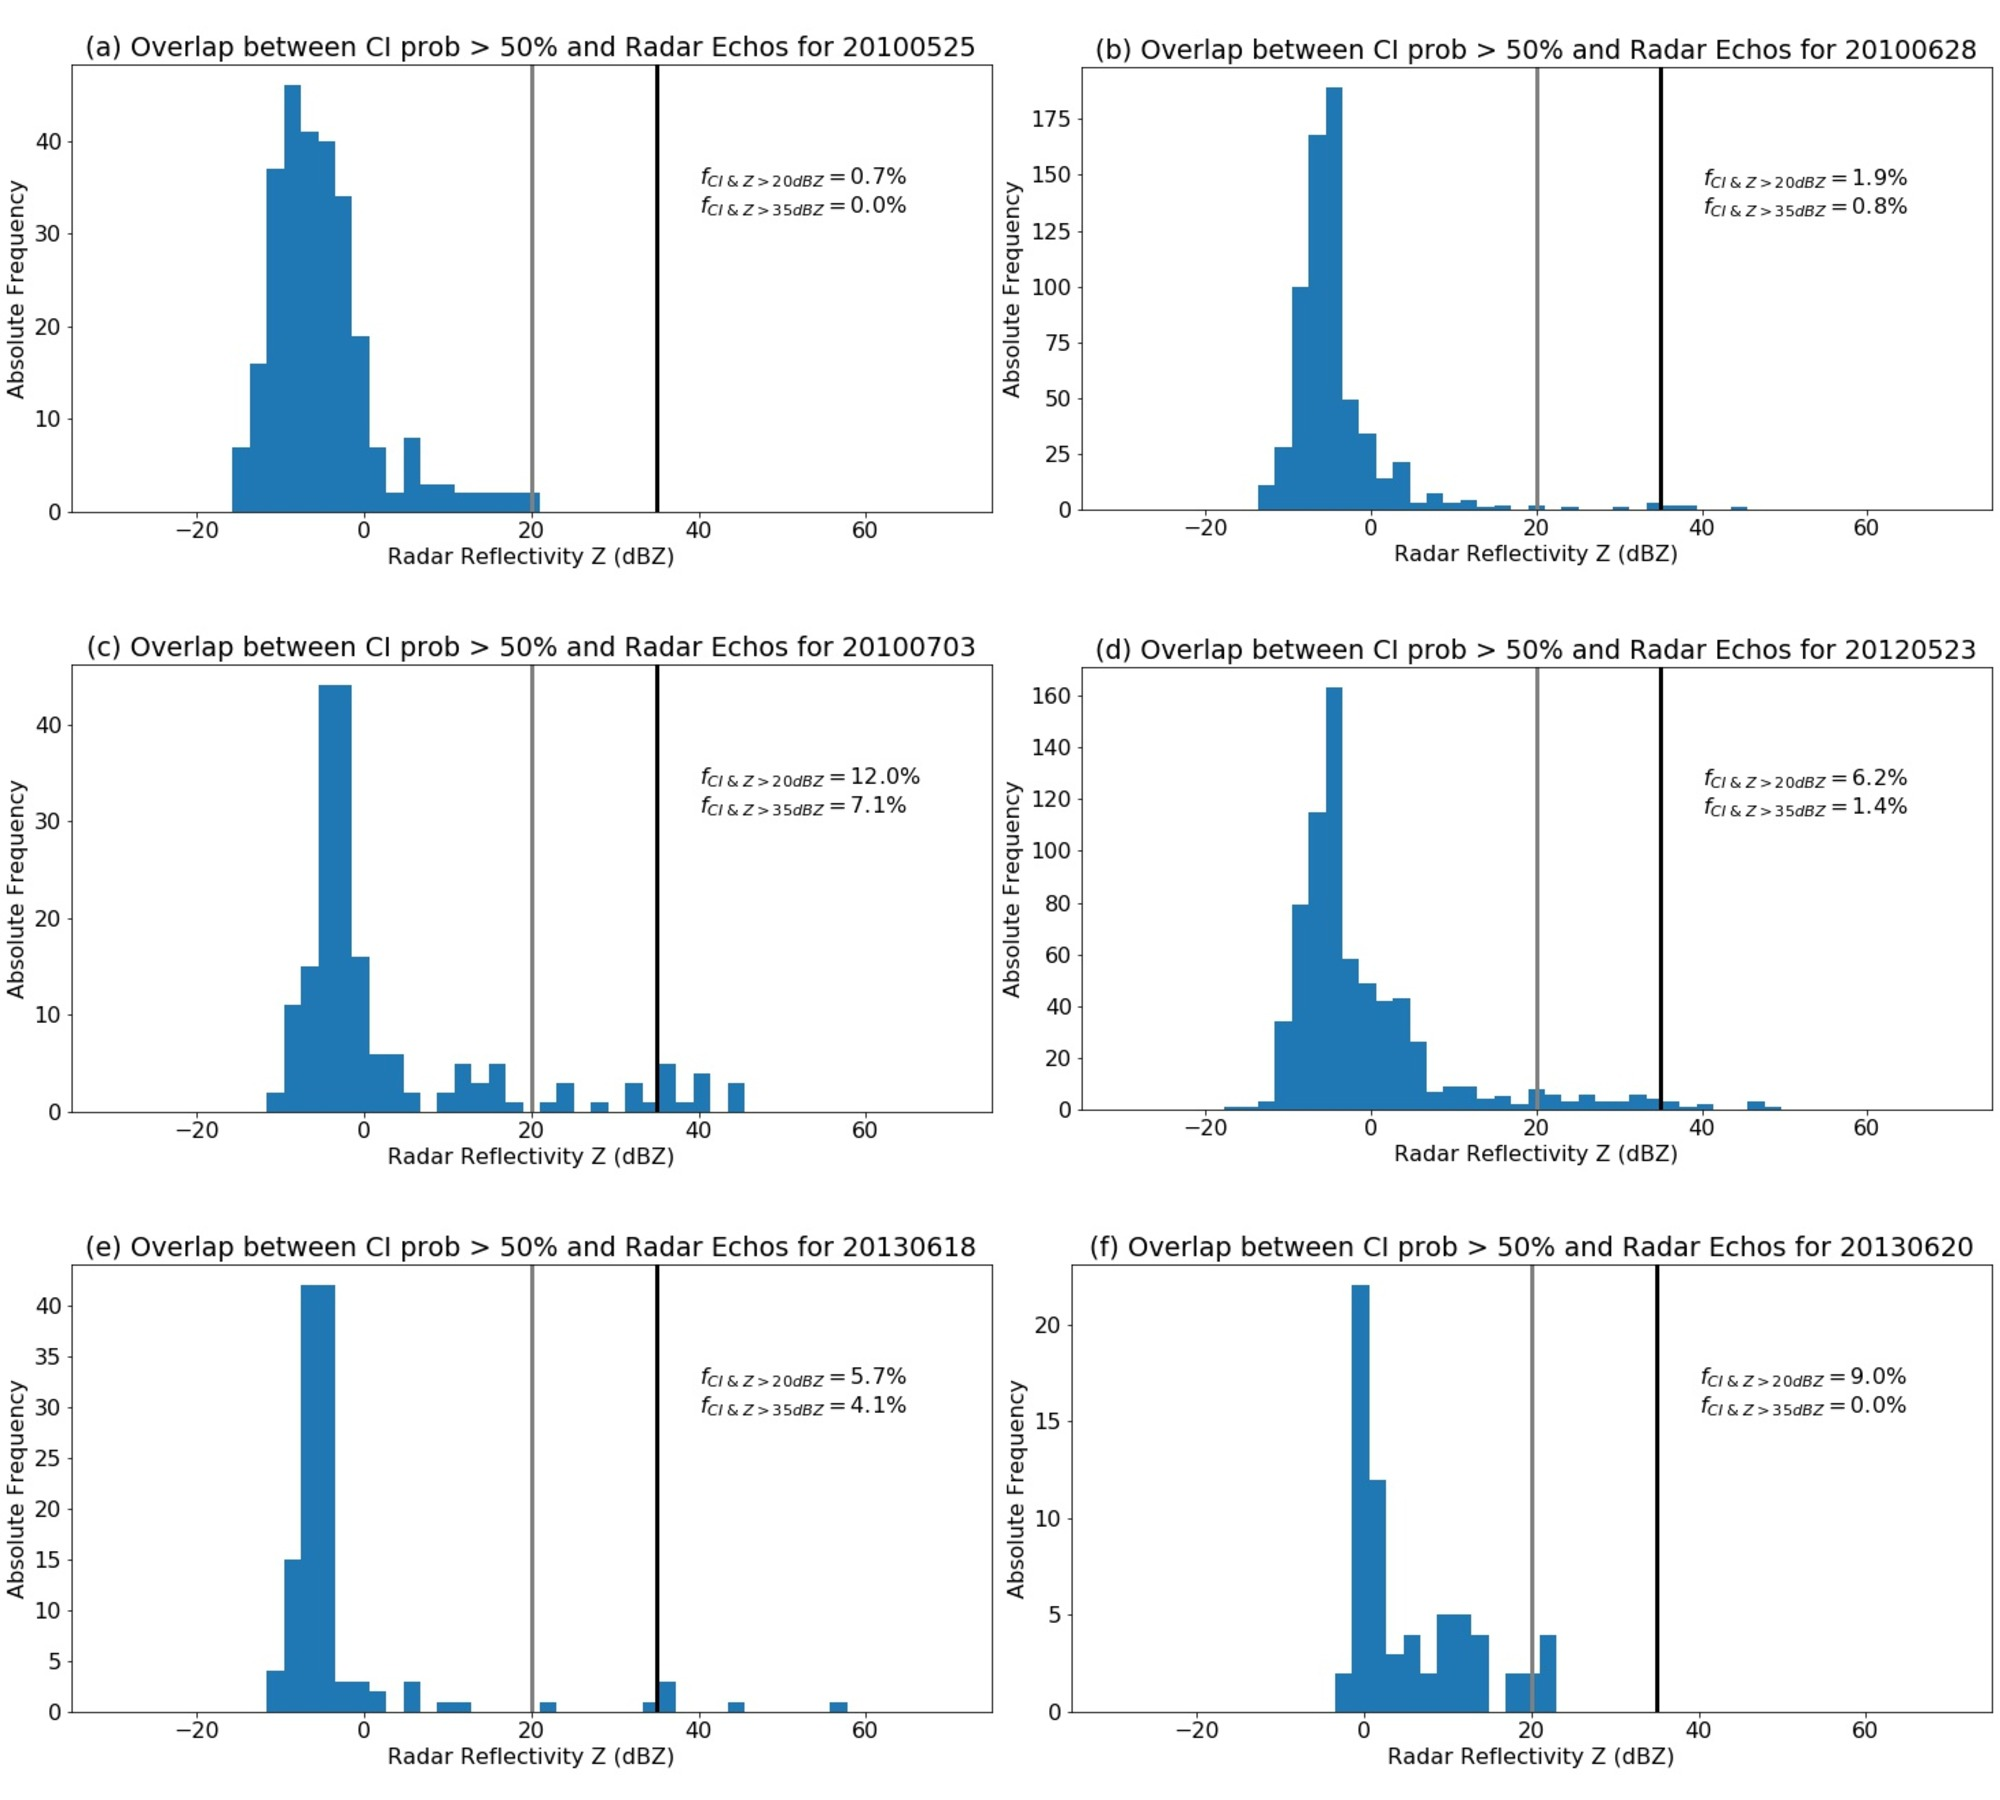
\includegraphics[width=\textwidth]{Grafiken/Abbildungen/overlap_CI50_RX.jpg}
\caption{Absolute Frequencies of radar reflectivities for CI detections with probability greater than 50\% for all six case days in chronological order (a) to (f). Two thresholds at 20 and 35 dBZ are marked with vertical lines.}
\label{fig:overlap_CI50-RX}
\end{figure}

A second analysis is again devoted to the question if CI detections occur in places where radar reflectivities are already large. Therefore, we measure the Euclidean distance between each of the CI pixels to the closest radar 35 dBZ contour. We excluded radar-derived objects smaller than 16 pixels to decrease sensitivity to false echoes and artifacts in the radar data. The absolute frequencies of distance counts are shown in Fig.~\ref{fig:distance_CI50-RX35}. It is hard to select a threshold distance at which a CI detection is considered to be too close to an existing precipitation event. If we select 15 km minimum distance, which is the buffer radius chosen for the radar object analysis, we see that in most of the cases only a small fraction of CI detection is closer than this distance. One exception is the distance statistic for the 23 May 2012. In this case, 22\% of the CI detections are very close to already existing precipitation. Please note that the distance analysis is very dependent on the CI object sizes and the general spatial distribution of the precipitation field.

\begin{figure}
\centering
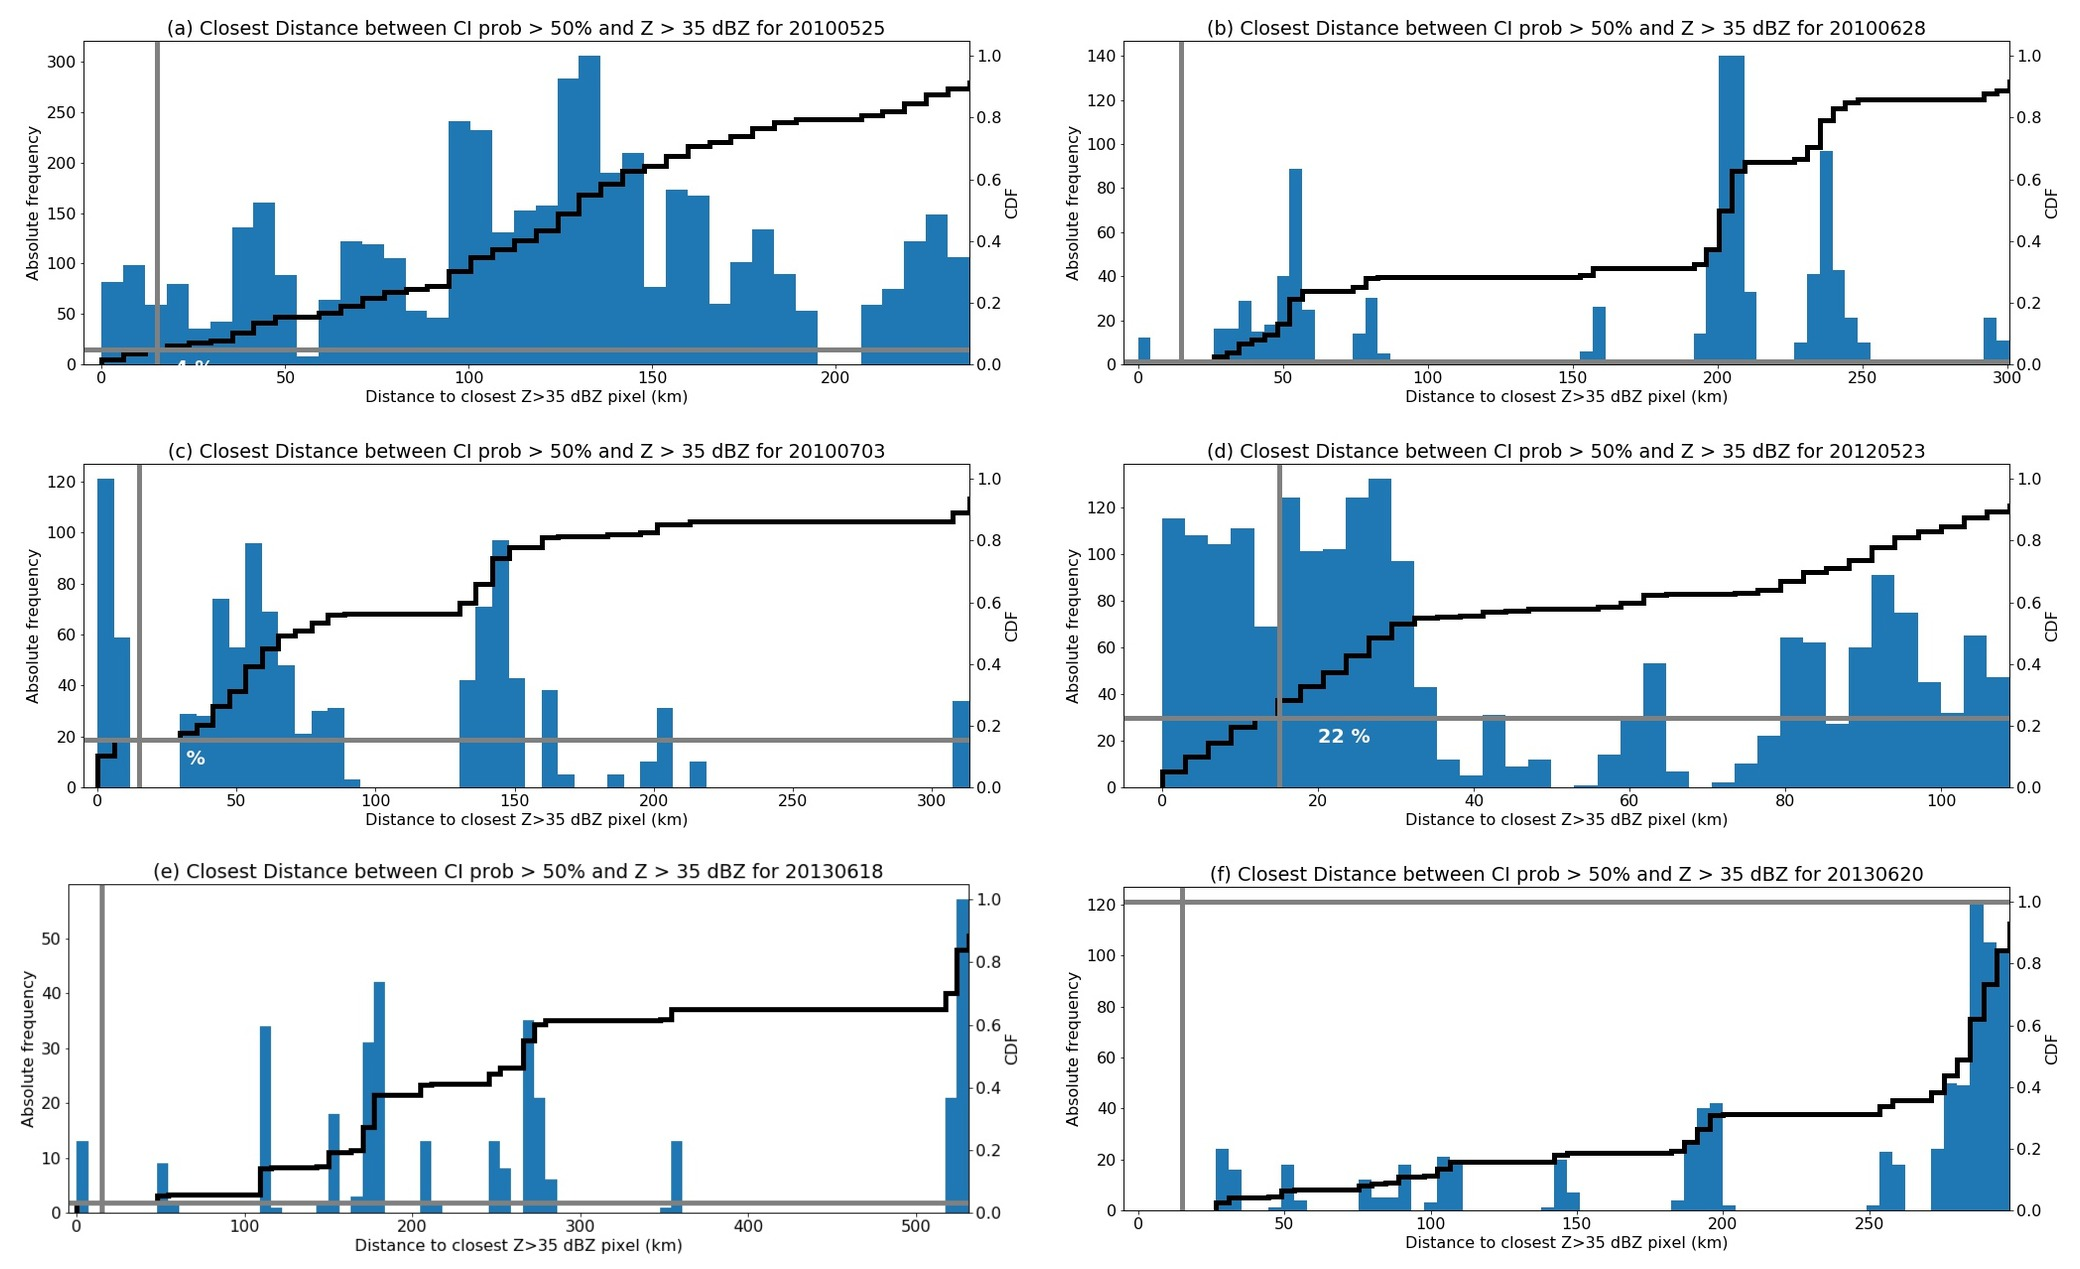
\includegraphics[width=\textwidth]{Grafiken/Abbildungen/distance_CI50_RX35.jpg}
\caption{Absolute Frequencies of distances to the closest 35 dBZ contour for CI detections with probability greater than 50\% (On each left y-axis, blue bars) for all six case days in chronological order (a) to (f). In addition, the panels shows the cumulative probability to have a 35 dBZ reflectivity contour closer than a certain distance (black solid lines).}
\label{fig:distance_CI50-RX35}
\end{figure}

\section{Temporal persistence of CI detections}
Also inspired by the provided cloud and precipitation movies, the question arises how long CI detections do last. Persistent CI detection indicate places where the probability for precipitation formation remains high. This is not  a problem on its own, and persistent CIs do not have to be false detections. However, if CI is issued with high probability at a certain place, one would expect for a high-quality detection, that precipitation will form within 30~min. A persistent CI that lasts more than 30\,min would not be appropriate in this case.

For the pixel-based analysis, we only consider the Eulerian perspective, i.e. we do not correct for the motion of clouds and their associated CI detections. As a first similar measure, we analyse spatial auto-correlation functions (see Fig.~\ref{fig:decorr_analysis}). CI fields with a small but fixed time lag have been compared with the help of linear pattern correlation coefficients. The resulting curve describes the de-correlation behaviour of the CI fields. Largest e-folding times with more than 75\,min are obtained for the 23 May 2012. For this case, long-lived cloud structures with a rather slow movement seem to imprint on the CI detections. For most of the other cases, the typical de-correlation time is between 15 and 30\,min indicating that CI detections are relative short lived. This is also a positive result, as the CI detection should be sensitive to a very narrow time interval within which the convective growth period lies, which occurs within 30 min or less \citep{Senf.Deneke_2017_JAMC}. 

\begin{figure}
\centering
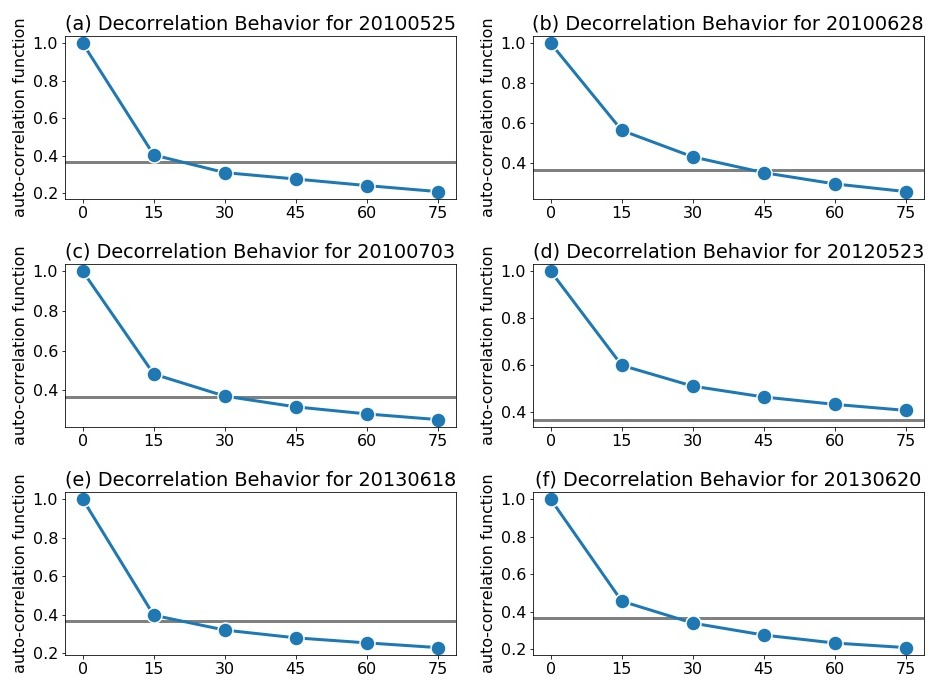
\includegraphics[width=\textwidth]{Grafiken/Abbildungen/decorrelation_CI.jpg}
\caption{Decorrelation analysis of the CI field for different case days from (a) to (f). Time-lagged pattern correlation coefficients have been calculated and averaged for one day. Grey line is at $\exp[-1]$ which marks the e-folding value. }
\label{fig:decorr_analysis}
\end{figure}

In a second exercise, we count how long each pixel is occupied by subsequent CI detections. This can be converted into a probability that a CI detection lives longer than a specified time interval. The results of this analysis are shown in Fig.~\ref{fig:life-time} for the low probability category $>25\%$. The figure shows that a relatively small fraction of the CI detection exhibits persistence. The probability for CI detections to live longer than 15~min lies between 10 and 20\%. Only a few percent of the CI detection live longer than 30~min.

\begin{figure}
\centering
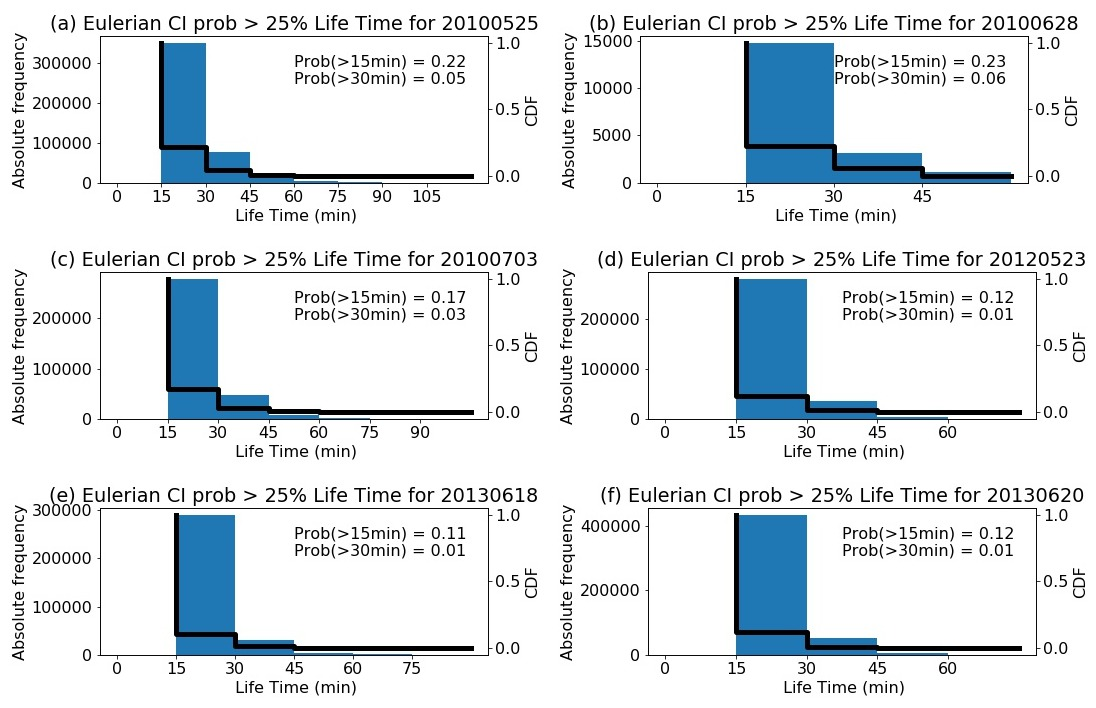
\includegraphics[width=\textwidth]{Grafiken/Abbildungen/life_time_CI25.jpg}
\caption{Eulerian life-time analysis of CI pixels in the category $>25\%$ for the different cases days.  Absolute frequencies of different life times are shown with blue bars, the probability that CI live longer than a certain time interval is given with black solid lines. }
\label{fig:life-time}
\end{figure}

For the higher probability CI categories, the situation is different: nearly all CI detections for and $>75\%$ live only one time step. These detection show no persistence. Thus, the de-correlation behaviour of the CI fields is dominated by the persistent character of the low probability CI events. Again, we recognise a very different behaviour of the low vs. high probability CI fields.

\section{Dominant cloud type of CI detections}
Another question inspired by the provided cloud and precipitation movies is which cloud type the CI detections have. Optimally, the CI detections should not be located in regions where there is no cloud or over cirrus clouds as cirrus cases are known to be problematic for CI detection algorithms . To analyse this, the NWC\,SAF v2013 cloud types of all CI detection pixels where collected for the 23\textsuperscript{rd} May 2012. 

As to be seen in Fig.~\ref{fig:ci_cloud_type}, the majority of CI pixels have expected cloud types .  More than \SI{90}{\percent} of the CI detections have a cloud type of very low, low and medium level clouds and fractional clouds, which makes sense. But there is also a small fraction having a cloud type of semi-transparent very thin clouds, which are cirrus clouds, and there is also a fraction of CI detections located over cloud free pixels.

Looking at the diurnal variation in the cloud type of CI detections Fig.~\ref{fig:ci_cloud_type_time}, it it becomes clear that the problem of CI detections with unexpected cloud types is linked to night times.  A likely explanation are differences in the version 2013 of the cloud type product used by TROPOS for this analysis and the version 2016 used by Meteo France for generating the CI product. Another possible option is, that there is a difference between the versions 2013, used in this analysis, and 2016, used for the CI product, of the NWC\,SAF cloud type product, especially in night time. But as this problem mainly effects the time span outside of the time frame used for the analyses of this study, no further investigation of this problem was conducted. 

\begin{figure}
\centering
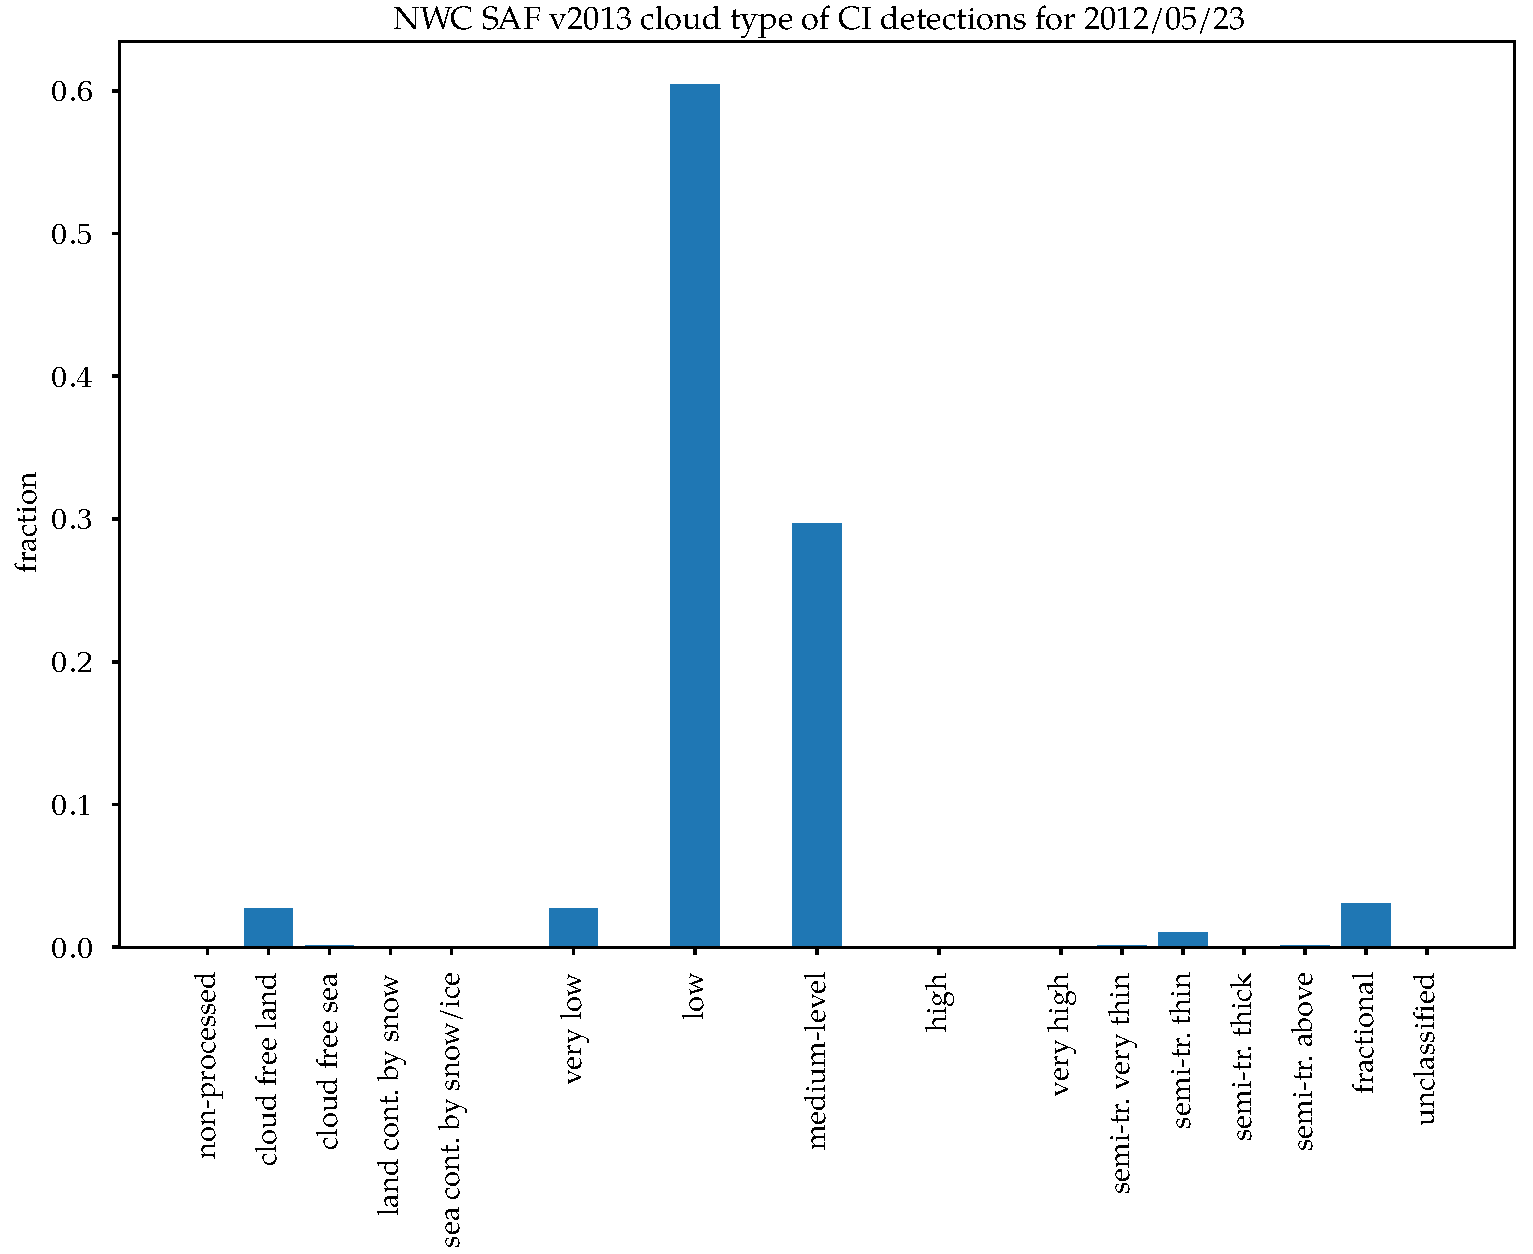
\includegraphics[width=0.9\textwidth]{Grafiken/Abbildungen/ci_cloud_types.pdf}
\caption{NWC\,SAF v2013 cloud types of CI detection pixels for 2012/05/23.}
\label{fig:ci_cloud_type}
\end{figure}

\begin{figure}
\centering
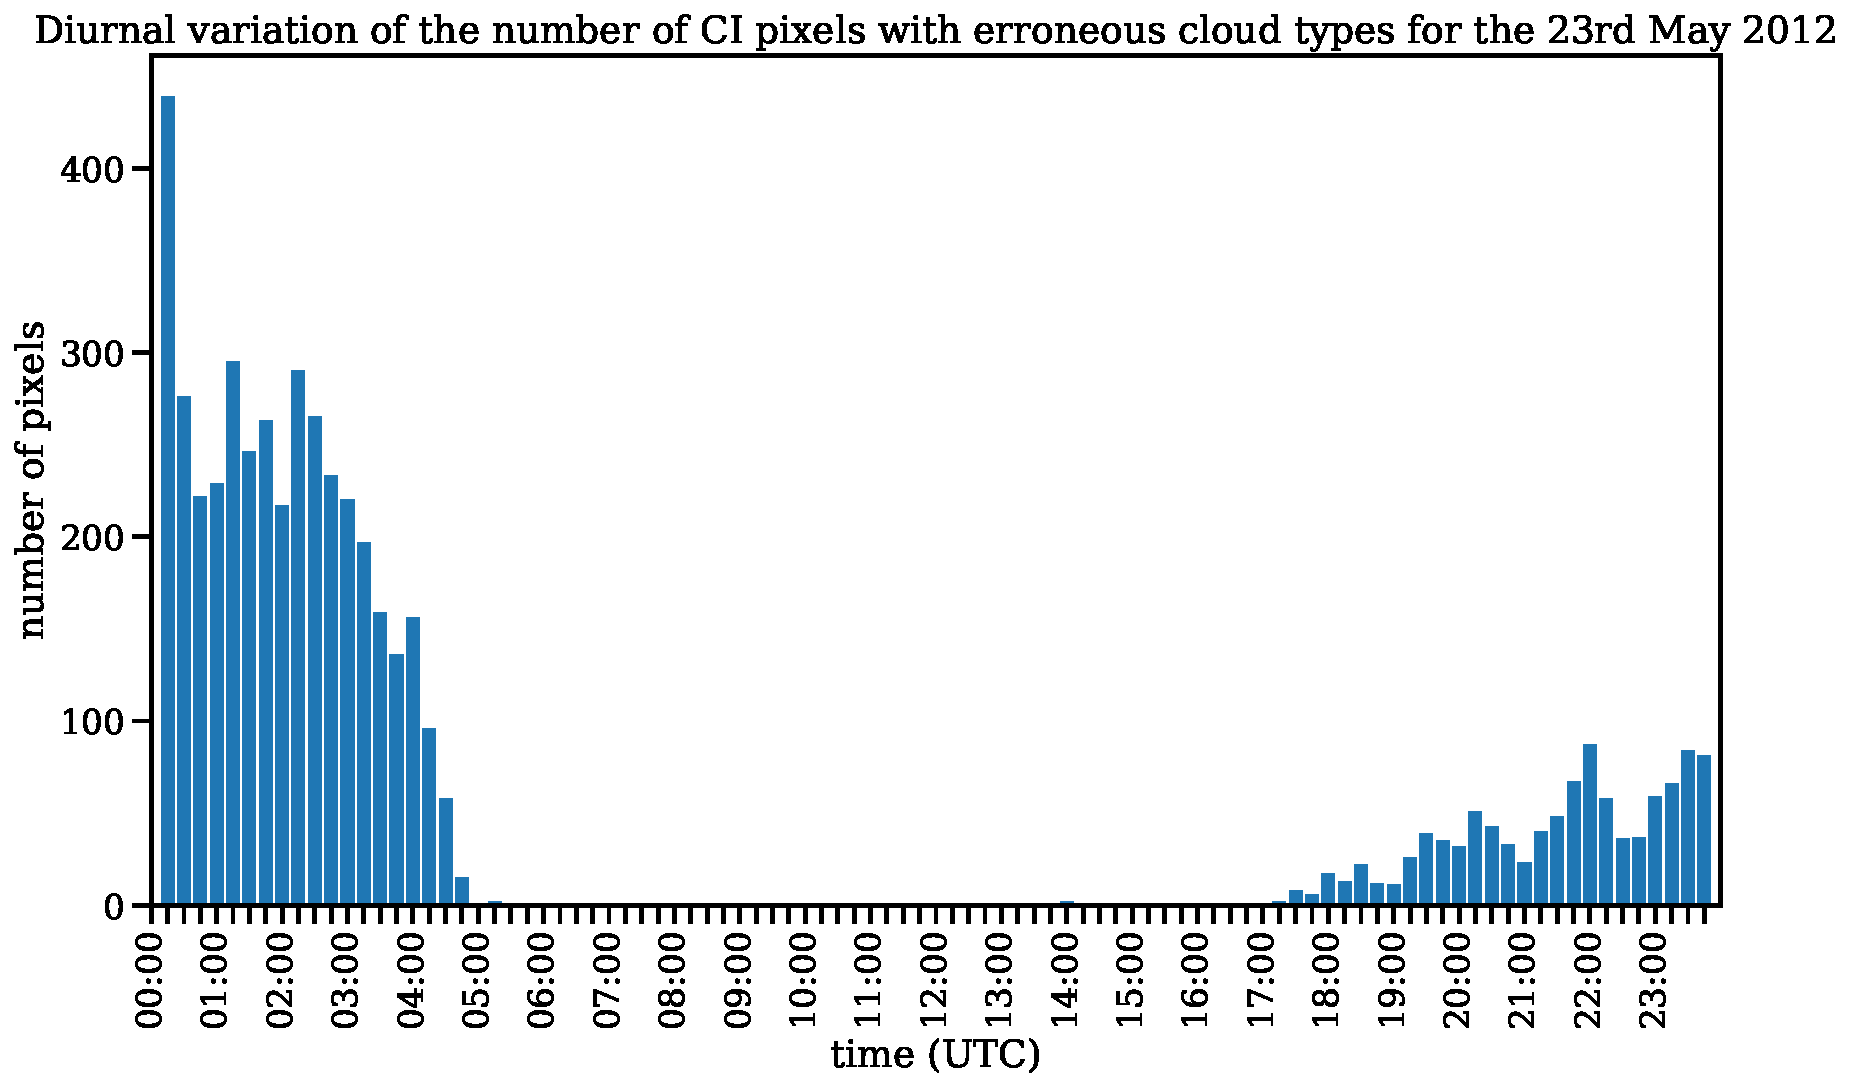
\includegraphics[width=0.8\textwidth]{Grafiken/Abbildungen/ci_cloud_types_time.pdf}
\caption{Diurnal variation of the number of CI detection pixels with erroneous cloud types for the 23\textsuperscript{rd} May 2012.}
\label{fig:ci_cloud_type_time}
\end{figure}
\chapter{Object-based Analysis}

\section{HRV cloud objects}
The derivation of cloud objects as described in Sec. \ref{sec:cloud} yielded a total of \num{1107} HRV cloud objects for the five case days, with \SI{80}{\percent} single cell objects and \SI{20}{\percent} complex objects, which are multi cell objects with a number of splits and merges. The vast majority of the single cell objects has only a rather short life time of \SIrange{15}{30}{\minute}, with a median life time of \SI{30}{\minute} (Fig.~\ref{fig:cell_ltime}). As  can been seen in Fig.~\ref{fig:cell_ltime}, the life time distribution for the complex objects is broader than the one for the single cells and the complex objects  have a longer life time with a median of \SI{60}{\minute}. There are no complex objects with a life time  lower than \SI{30}{\minute}  due to the definition of the complex objects.  At least two time steps are needed to develop splits or merges, so that the minimum life time of these objects is at least \SI{30}{\minute}. The multi-cell objects can be quite complex, with up to \num{26} splits or merges in one object (Fig.~\ref{fig:splits_merges}). Such objects typicallyrepresent large compact cloud fields which usually are present for a longer time . But most complex objects have only have very few splits or merges, with a median value of one split or merge. These objects mainly represent smaller cloud objects, which grow together to form larger objects. Splits and merges are roughly similarly abundant, but splits are a bit more frequent in the objects than merges. One reason for this is that the rather large and long living cloud fields tend to dissolve on the boundaries and  create smaller objects that do not merge again.

Separating the complex objects at the split and merge points, and only conserving the objects prior to these points, an additional number of \num{2915} single cells can be derived. The life time distribution of the single objects derived from the complex objects is quite similar to the distribution of the single cell objects (Fig.~\ref{fig:single_cell}).

When only taking into account all single cells with a life time of at least \SI{30}{\minute}, to be consistent with the ground truth definition, the number of eligible objects decreases to \num{1584} objects. Additionally, not all the validation area is covered by the radars, and only the objects inside the radar-covered area can be used for the validation. This reduces the number of eligible objects further to 1180. The subsequent analysis was conducted with these objects.

\begin{figure}[htbp]
\centering
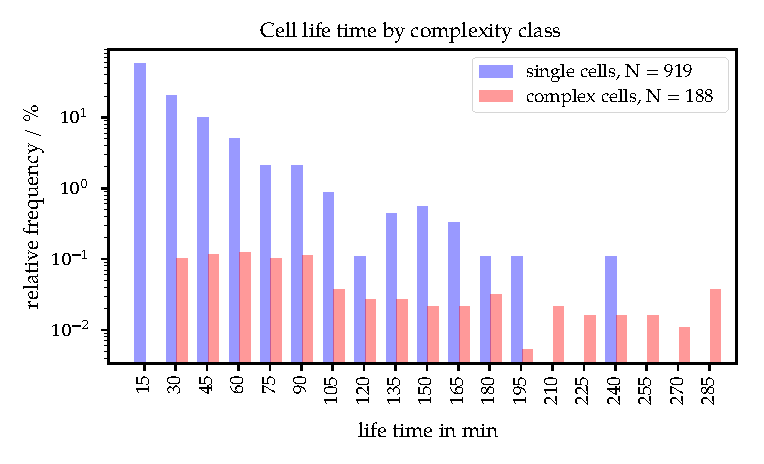
\includegraphics[width=\textwidth]{Grafiken/Abbildungen/cellclass_lifetime.pdf}
\caption{Comparison of the life time of single (blue) and multi cell (complex) objects (red).}
\label{fig:cell_ltime}
\end{figure}

\begin{figure}[htbp]
\centering
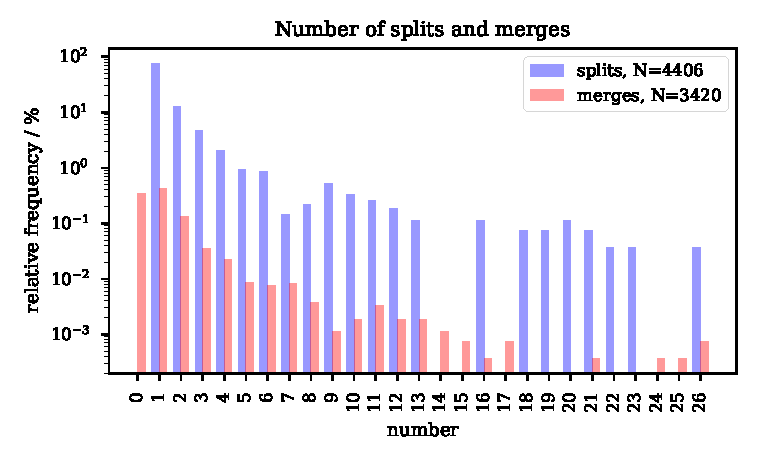
\includegraphics[width=\textwidth]{Grafiken/Abbildungen/splits_merges.pdf}
\caption{Distribution of number of splits and merges in the complex objects.}
\label{fig:splits_merges}
\end{figure}

\begin{figure}[htbp]
\centering
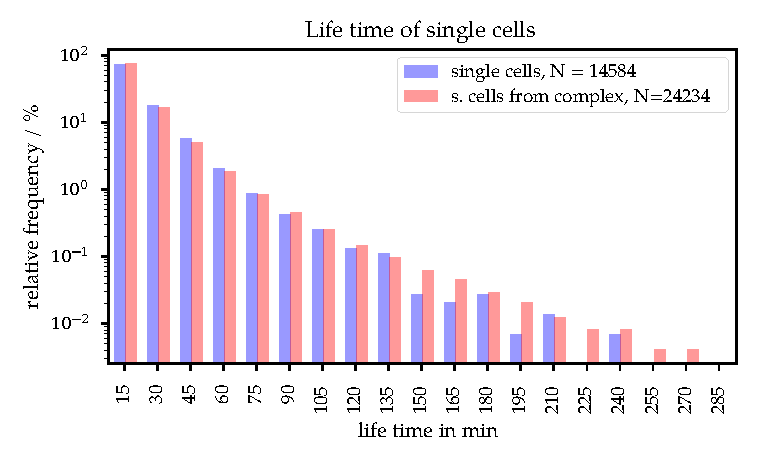
\includegraphics[width=\textwidth]{Grafiken/Abbildungen/single_from_complex_lifetime.pdf}
\caption{Comparison of the life time of single cell objects (blue) and the single cell objects derived from complex objects (red).}
\label{fig:single_cell}
\end{figure}

\section{Ground truth objects}
Using the weather radar data and applying the approach presented in Sec. \ref{sec:haci}, \num{526} ground truth objects with a minimum life time of \SI{30}{\minute} could be derived in the time frame 05:00 am UTC to 05:00 pm UTC for the six case days. This number is only around \SI{53}{\percent} of the number of cloud objects,  as not all clouds form precipitation. 

As it can be seen in Fig. \ref{fig:haci_frequency}, the proportion of the number of ground truth objects is quite variable for the case days. Most of the ground truth objects stem from the three case days 3\textsuperscript{rd} July 2010, 23\textsuperscript{rd} May 2012 and 20\textsuperscript{th} July 2013, which account for more then \SI{80}{\percent} of all ground truth objects. 

As is also visible from Fig. \ref{fig:haci_frequency}, the ratio of ground truth objects matching with at least one cloud object is almost or equal to \SI{100}{\percent} for  most case days. The only exception is 28\textsuperscript{th} June 2010 where the ratio lies a bit above \SI{60}{\percent}. This day is also the day with the highest percentage of cloud objects, with around \SI{30}{\percent} of all cloud objects having been derived from this day. On this case day, there is convective development over large parts of Germany with the exception of the North-East. Most of the convective developments are rather isolated, leading to the rather high percentage of cloud objects coming from this day. But  most of these cells do not form precipitation. Convective cells forming precipitation start to develop along and downstream of the Black Forest in South West Germany and the Vosges Mountains in Eastern France. But these cells exhibit rather complex developments and thus are missed by our cloud object derivation approach.  For the other case days, our cloud object approach works quite well and captures the most prominent developments.

\begin{figure}[htbp]
\centering
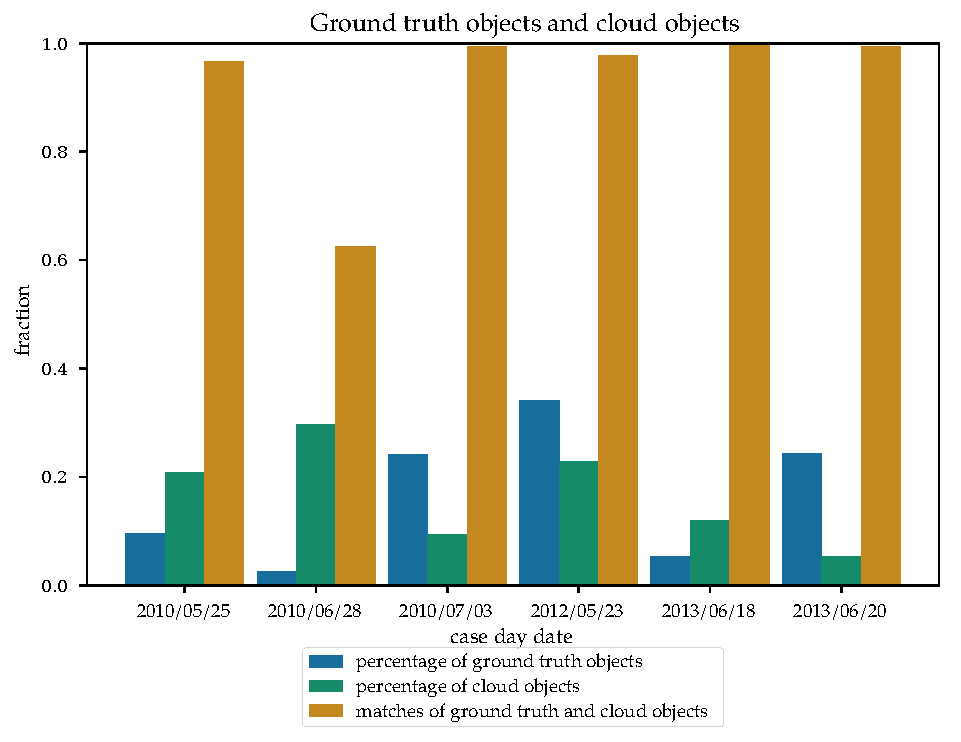
\includegraphics[width=\textwidth]{Grafiken/Abbildungen/haci_hrv_frequencies.pdf}
\caption{Proportion ground truth objects of the case days to the total number of ground truth objects (blue), proportion of cloud objects to total number of cloud objects, (green) and proportion of ground truth objects matching with cloud objects (yellow).}
\label{fig:haci_frequency}
\end{figure}

\section{Validation results}
The validation of the \SI{30}{\minute} forecast of the NWC\,SAF CI product v2018 using the approach presented above yields the validation statistics given in Fig.~\ref{fig:validation_result1} and Tab.~\ref{tab:validation_result}. Although the number of cases used for the validation seems sufficiently large, only two of the CI probability levels can be evaluated, as there are only true positive cases for the levels \SIrange{25}{50}{\percent} and \SIrange{75}{100}{\percent}. For all CI probability levels, the vast majority of cases are true negative cases. True positives, false positive and false negative seem to be quite randomly and unequally distributed over the CI probability levels. The total number of true positive cases sums up to only 15 cases, with ten for level \SIrange{25}{50}{\percent} and five for level \SIrange{75}{100}{\percent}. So the validation results are statistically not very robust and need to be interpreted cautiously. 

\begin{table}[htb]
\centering
\caption{Confusion matrix for the validation result}
\begin{tabular}{cccc} 
\toprule
\multirow{2}{*}{CI product detection} &     & \multicolumn{2}{c}{weather radar detection} \\
							   						  \cmidrule{3-4}
									  &     &  yes & no \\
\midrule
\multirow{2}{*}{level 1}  & yes &    0 &    1 \\
	                                  & no  &   14 & 1157 \\ 
\midrule
\multirow{2}{*}{level 2}  & yes &   10 &   31 \\ 
	                                  & no  &    9 & 1125 \\ 
\midrule	                                  
\multirow{2}{*}{level 3}  & yes &    0 &    2 \\ 
	                                  & no  &   14 & 1156 \\ 
\midrule	                                  
\multirow{2}{*}{level 4}  & yes &    5 &    5 \\ 
	                                  & no  &   13 & 1152 \\
\addlinespace
\bottomrule
\end{tabular}
\label{tab:validation_result}
\end{table}

One reason for this is, that, as shown in Section~\ref{sec:diurnal_cycle} co-occurences of CI detections with radar reflectivity factors of more or equal to \SI{35}{dBZ} are quite rare. Thus, our validation approach of using objects based on a radar reflectivity factor of \SI{35}{dBZ} is rather strict and ensures that the rate of false detections is not increased artificially.

As visible in Fig.~\ref{fig:validation_result2}a, the two levels for which true positives are existing behave quite differently in terms of POD and FAR. The lower CI probability level has a rather high POD of \num{0.52} but also a quite high FAR of \num{0.76}. As to be expected, the higher CI probability level exhibits a lower POD of a  \num{0.28} but also a lower FAR of 0.50.

%Taking into account the distribution of the CI detections over the case days (Fig.~\ref{fig:validation_case_days}), it has to be noted that the contribution of the different case days to the validation result is quite different. So, the most true positives come from the 23\textsuperscript{rd} May 2012 while there are no true positives on 28\textsuperscript{th} June 2010. In fact the distribution of true positives for the case days looks quite similar to the distribution of ground truth objects in Fig.~\ref{fig:haci_frequency}} and the distribution of false positives looks quite similar to the distribution of cloud objects. So the result of the study is probably influenced by the number of available objects to be evaluated and thus the validation  is statistically not very robust. A higher number of case days could probably eliminate this behaviour. Moreover, there are no false negatives for the first three case days while the second three case days have them. This can be an indication that the algorithm of the NWC\,SAF CI product works better for certain weather patterns than for others. On the first three case days the convective development started over over France or the border region between France and Germany and than moved inside the study area. On the second three case days the convective development started within the study area. So, differences in meteorological and also geographical conditions can be causes for this different behaviour in the false negative cases. But, as the NWC\,SAF product has been mainly tuned over France, there is also the possibility that the algorithm parameters work best over France and have to be re-calibrated for different regions and different meteorological conditions. This should be investigated further in future studies concerning the NWC\,SAF CI product.

Taking into account the number of CI detections for the case days (Fig.~\ref{fig:validation_case_days}), it has to be noted that the contribution of the different case days to the validation result is quite different. Most true positives come from the 23\textsuperscript{rd} May 2012, while there are no true positives on 28\textsuperscript{th} June 2010. In fact the distribution of true positives for the case days looks quite similar to the distribution of ground truth objects in Fig.~\ref{fig:haci_frequency} and the distribution of false positives looks quite similar to the distribution of cloud objects. So the result of the study is probably influenced by the number of available objects to be evaluated and thus the validation  is statistically not very robust. A higher number of case days could probably help to address this behaviour. Moreover, there are no false negatives for the first three case days in contrast to the second three case days. This can be an indication that the algorithm of the NWC\,SAF CI product works better for certain weather patterns than for others. On the first three case days, the convective development started over France and the border region between France and Germany, and then moved inside the study area. On the second three case days, the convective development started within the study area. So, differences in meteorological and geographical conditions could be causes for this different behaviour. But as the NWC\,SAF product has been mainly tuned over France, there is also the possibility that the algorithm parameters work best over France and have to be re-calibrated for different regions and different meteorological conditions. This aspect should be investigated further in future studies

Considering the CSI (Fig.~\ref{fig:validation_result2}b) the two CI probability categories {lie} in the same range, with a value of \num{0.19} for \SIrange{25}{50}{\percent} CI probability, and \num{0.21} for \SIrange{75}{100}{\percent} CI probability. This means that only around one fifth of really occuring events were correctly forecast , with the higher CI probability showing a slightly higher skill. 

For the HSS the picture looks similar. The higher CI probability category again has a higher prediction skill, with an HSS value of \num{0.31}, whereas the lower CI probability category has an HSS of \num{0.34}.  Both values lie above 0, indicating a skill to forecast an event better than chance. Also, both HSS values are higher than the CSI values, implying that the strength of the forecast is more on the side of correctly predicting true negatives, which is not taken into account in the CSI.


\begin{figure}[htbp]
\centering
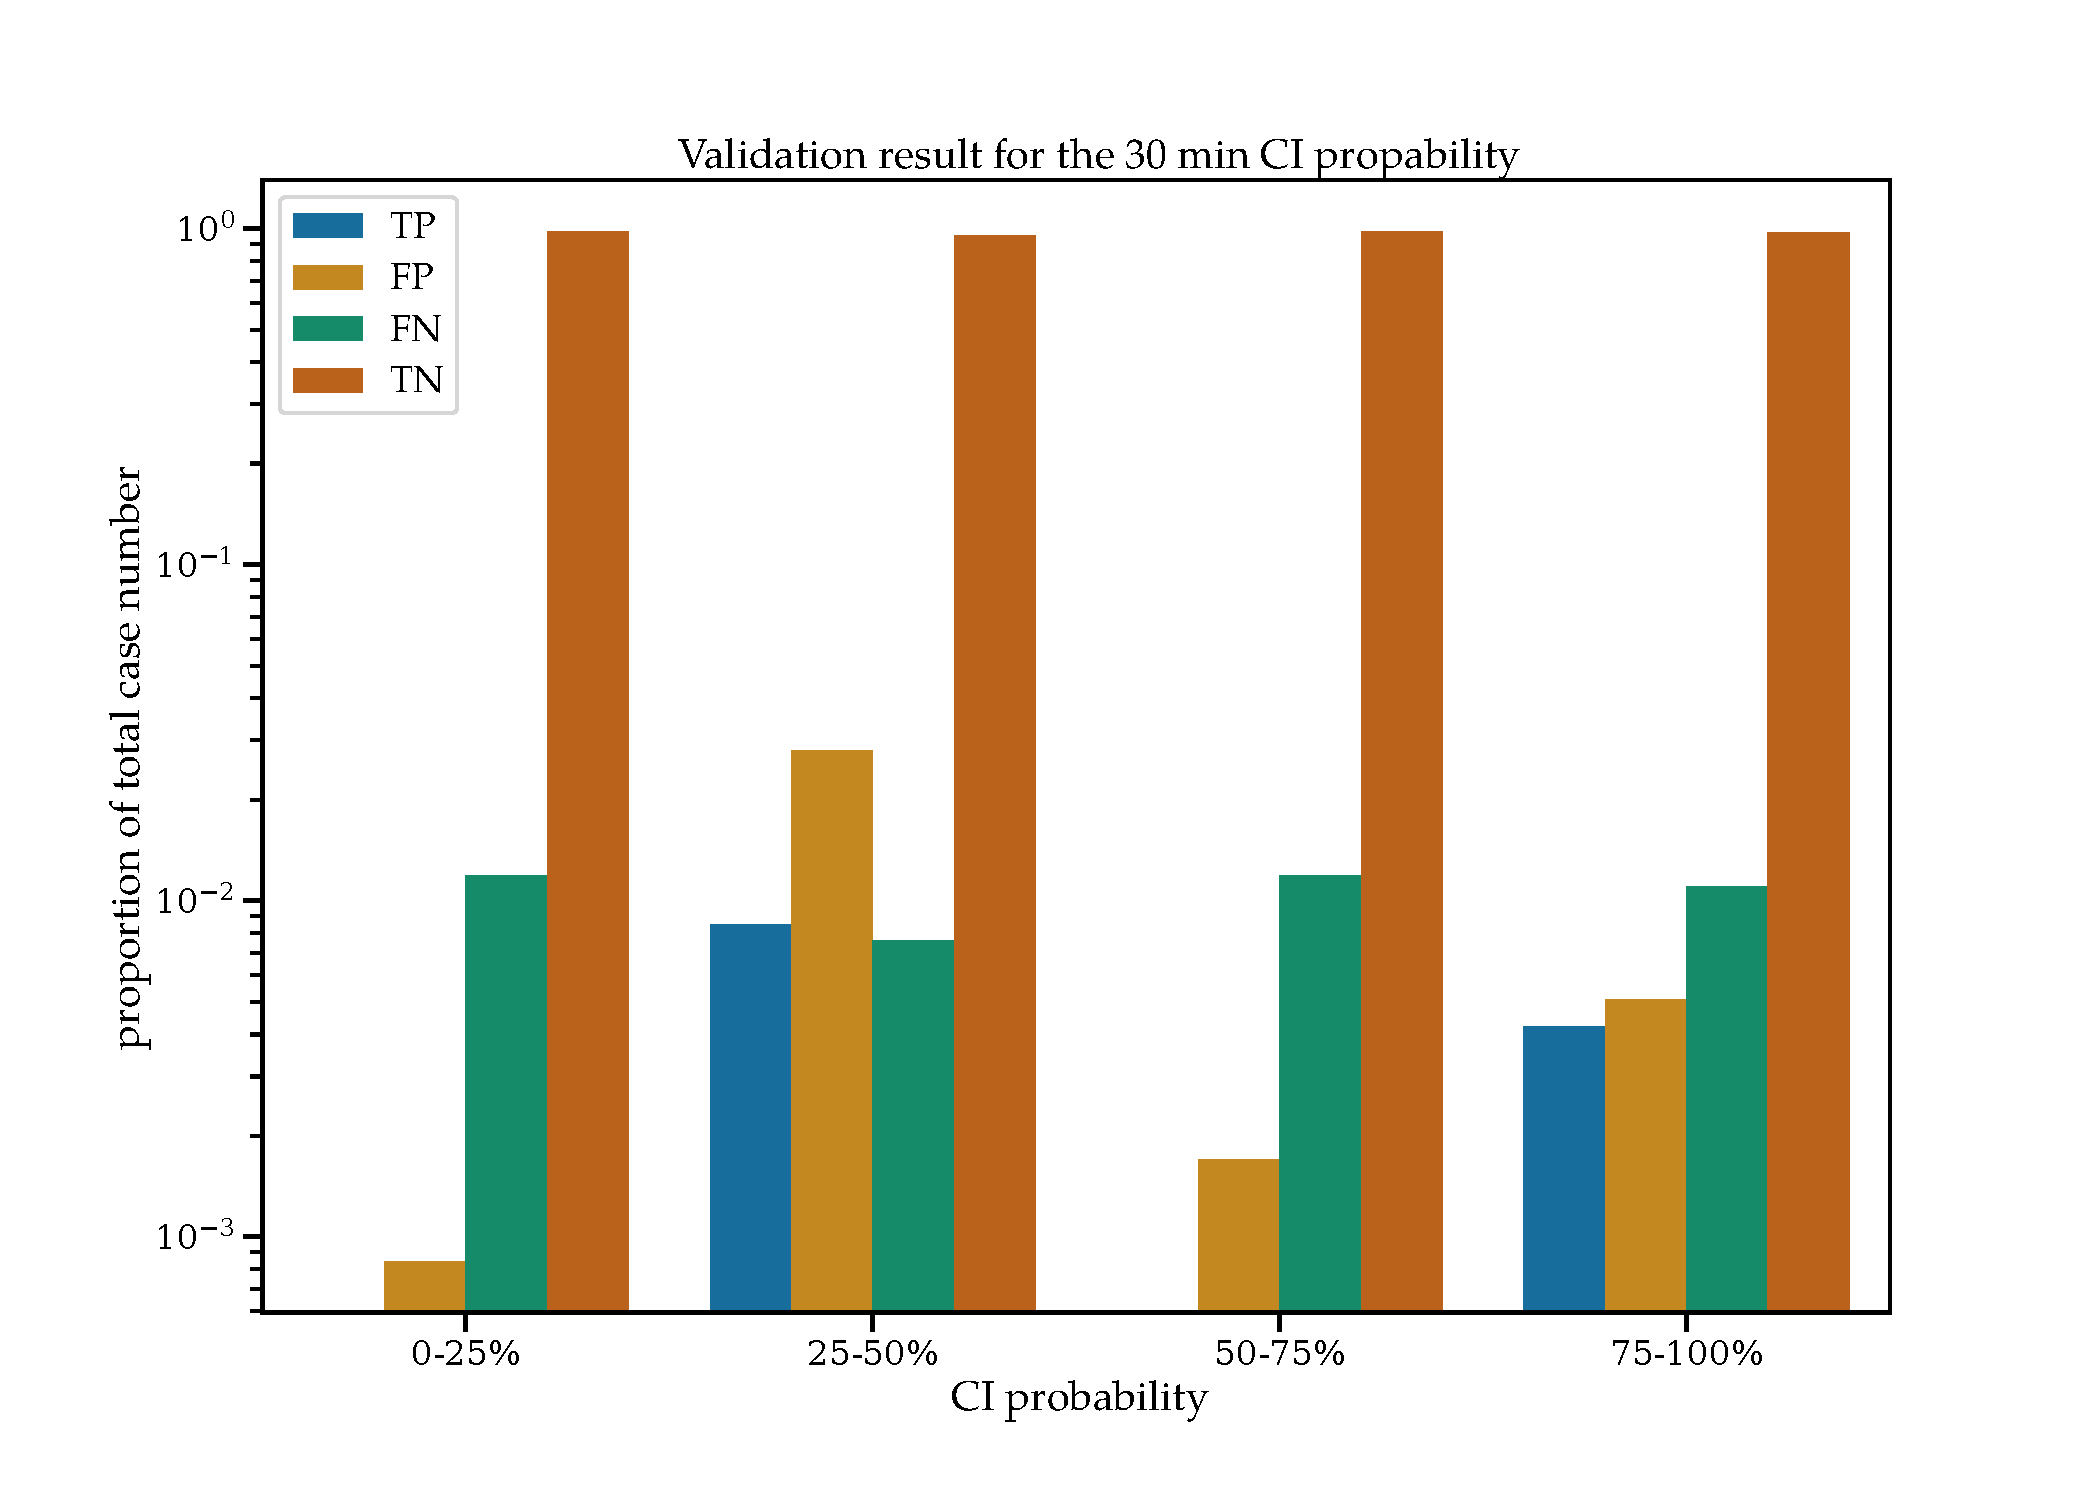
\includegraphics[width=0.8\textwidth]{Grafiken/Abbildungen/validation_plot.pdf}
\caption{Validation results for the \SI{30}{\minute} CI probability. Given are the proportion of true positives (FP, blue), false positives (FP, yellow), false negatives (FN, green) and true negatives (TN, orange) relative to the total number of cloud objects. Please note, that the abscissa is logarithmic.}
\label{fig:validation_result1}
\end{figure}

\begin{figure}[htbp]
\centering
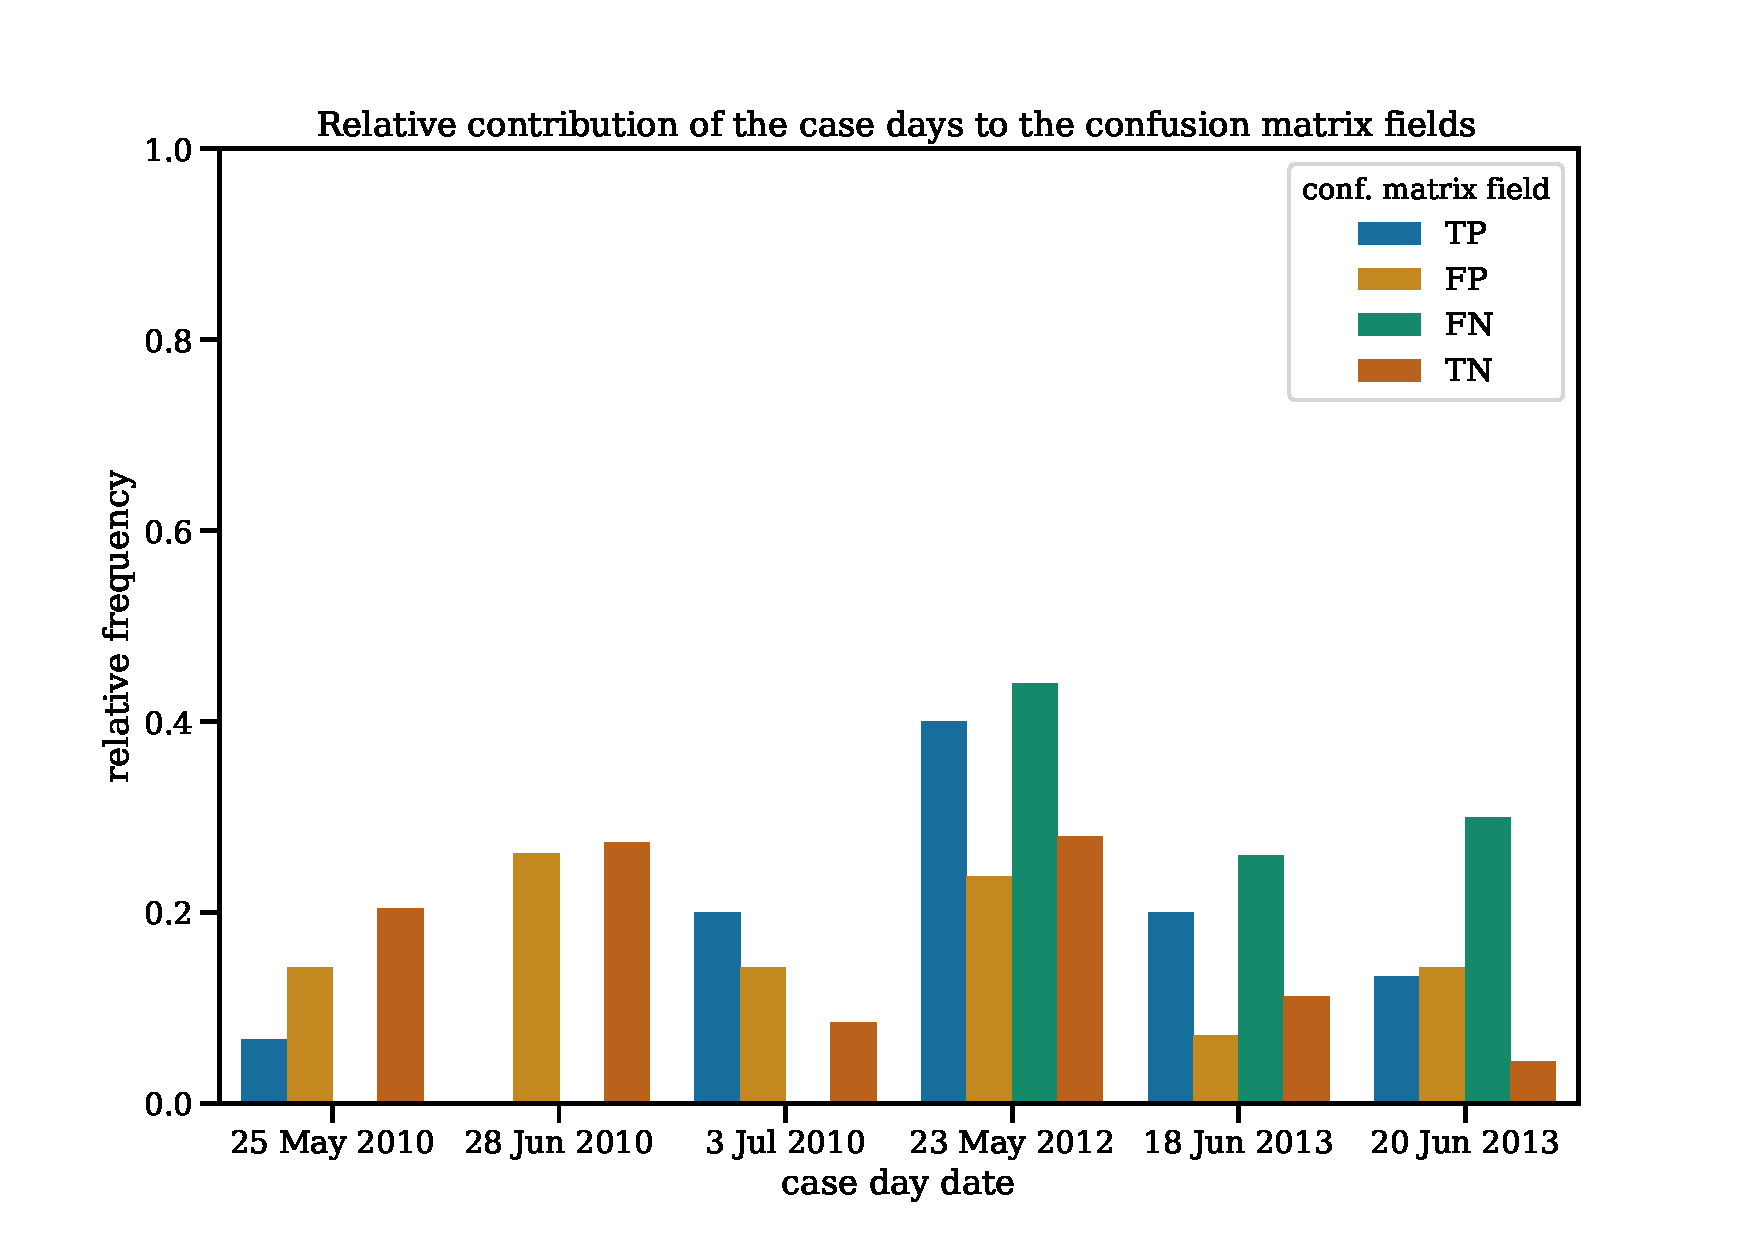
\includegraphics[width=0.8\textwidth]{Grafiken/Abbildungen/validation_case_day_frequencies.pdf}
\caption{Contribution of case days to the fields of the confusion matrix. Given is the relative proportion of cases per case day contributing to true positives (TP, blue), false positives (FP, yellow),false negatives (FN, green) and true negatives (TN, orange).}
\label{fig:validation_case_days}
\end{figure}


\begin{figure}[htbp]
\centering
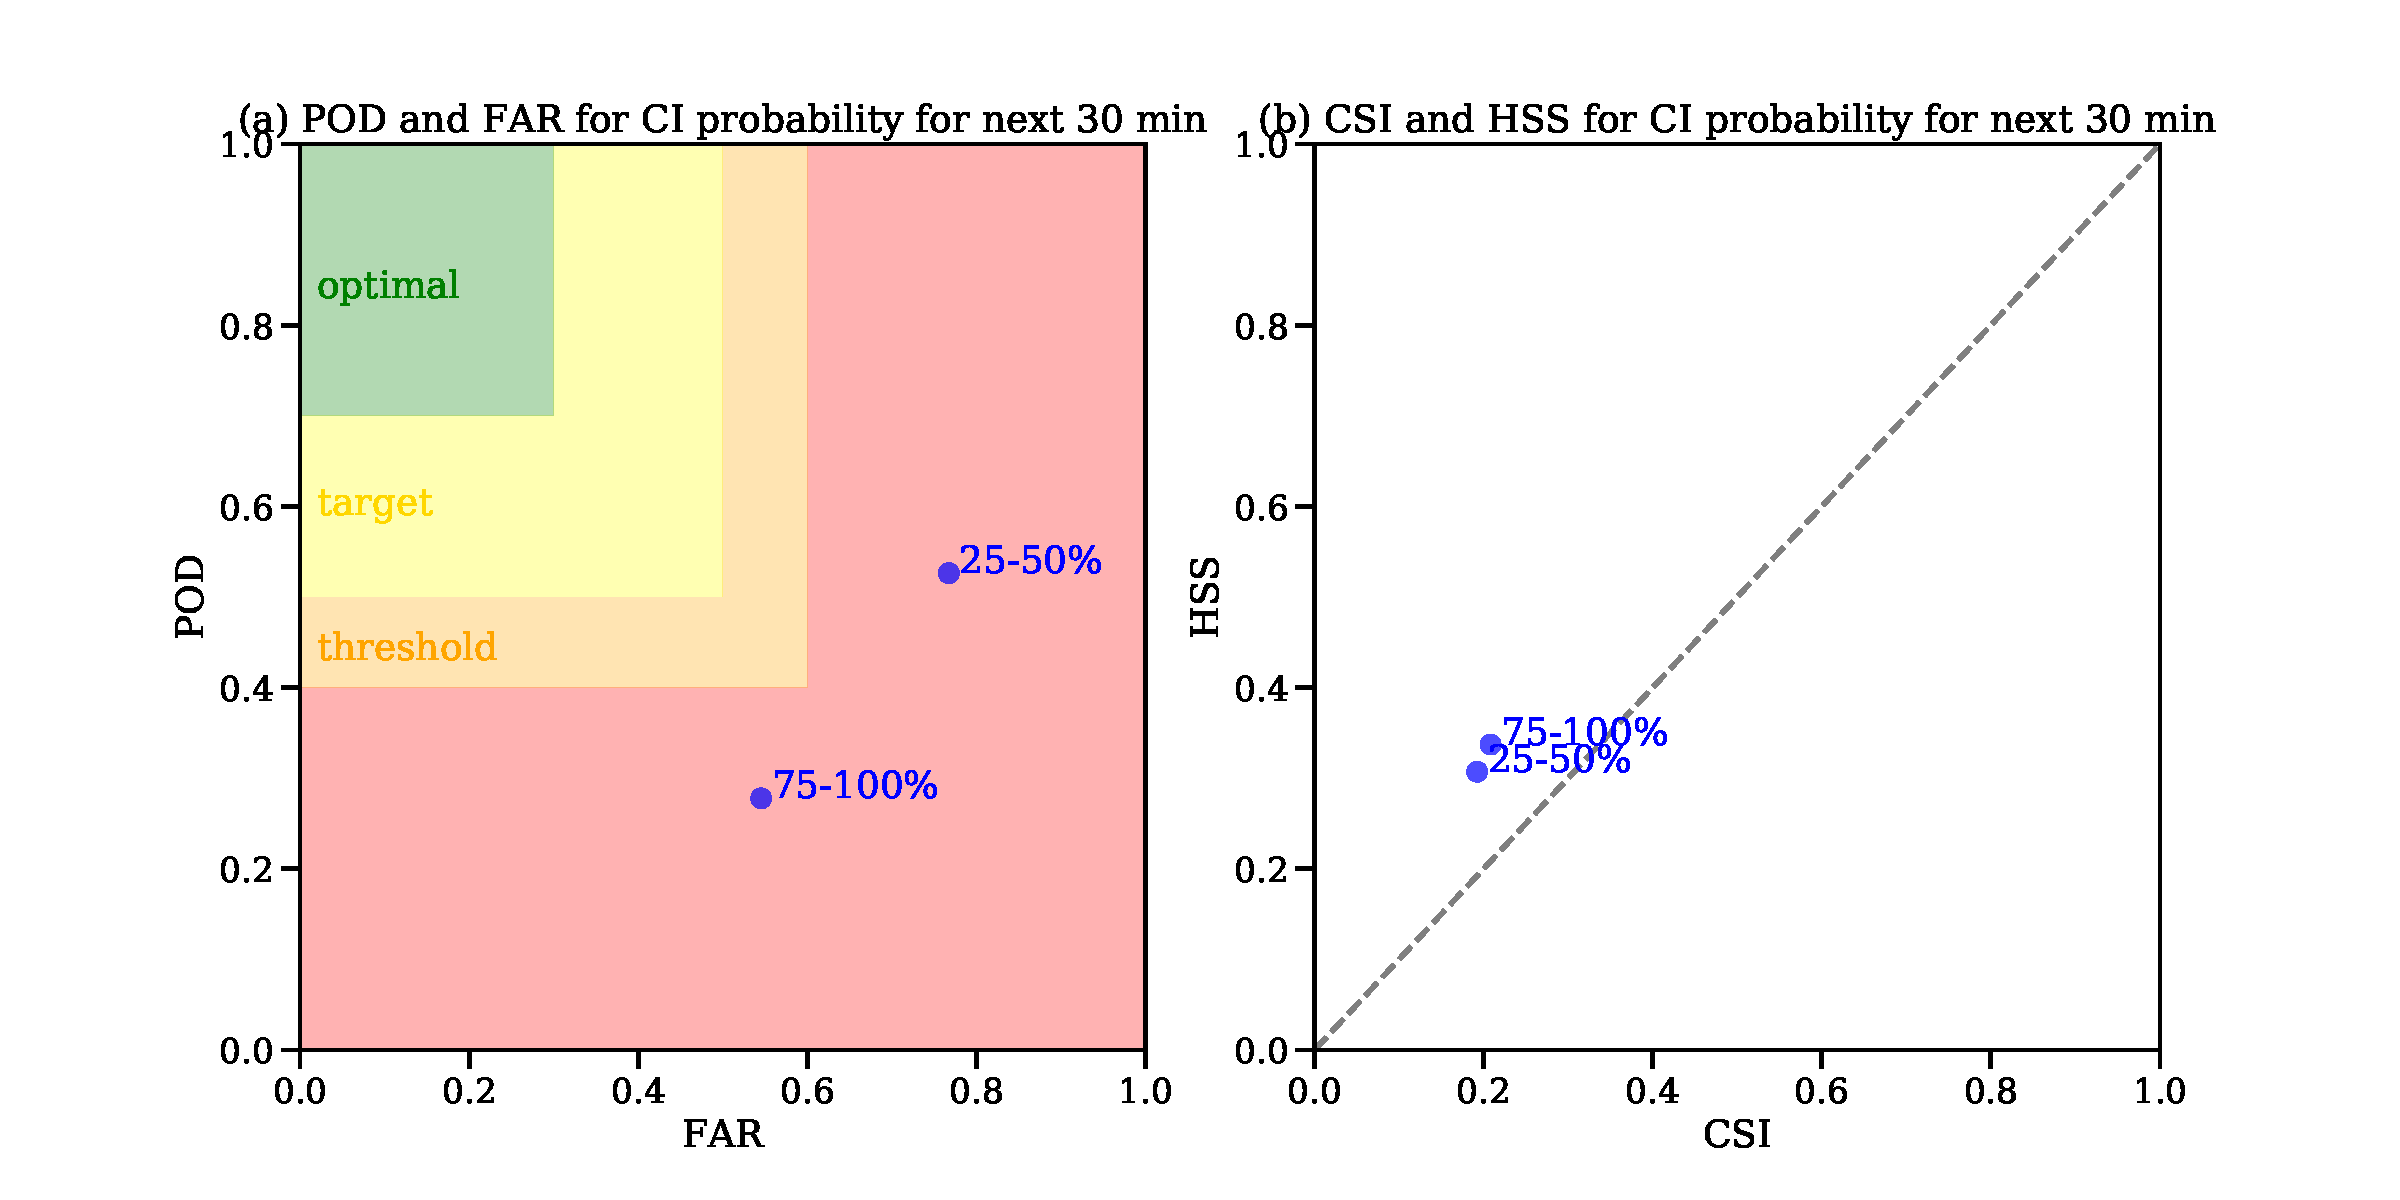
\includegraphics[width=\textwidth]{Grafiken/Abbildungen/validation_far_pod_hss_csi_plot.pdf}
\caption{Plot of the POD and FAR  and CSI and HSS of the validation of the CI product for the different CI probability levels. The colour surfaces in (a) denote the levels of POD and FAR given by the EUMETSAT requirements.}
\label{fig:validation_result2}
\end{figure}





\chapter{Conclusion and Recommendations}

This report summarises the investigations carried out in the framework of this NWC\,SAF associate scientist activity, which was targeted at the validation of the v2018 CI product. 

A number of methodological improvements have been made over the previous validation, which include the following: 1) using motion fields to forecast the future location of CI events and thus enable a more meaningful validation with radar observations used by us as ground truth in this study; 2) parallax-correction of the satellite-based products to achieve better overlap with the radar observations used as ground truth; 3) a first attempt towards an object-based evaluation of the product. 

In the first result chapter (Chapter 4), several field-based analyses have been presented. First, the diurnal cycles of the total areal coverage of the CI product have been contrasted with the areal coverage of the raining area obtained from ground-based radar. The comparison reveals a rather different behaviour of the CI product at different probability levels. The low-probability classes with a probability less than 50\% cover a significant areal fraction of the validation domain for the case days and show little correspondence to the diurnal cycle of the areal coverage of rain areas obtained from radar. This suggests a too-high sensitivity and poor discriminative skill for convective development of the low-probability classes.
In contrast, a much smaller areal coverage and a direct correspondence of the high-probability classes to subsequent increases in precipitating area have been found for the high-probability classes. 
Two additional consistency aspects of the CI product have been investigated: CI warnings should not include regions with existing significant precipitation, and due to the definition of CI, temporal persistence of warnings should generally not exceed the forecast horizon of the CI product. Both aspects were found to be satisfactory for the high-probability levels , while deficiencies were noted for the lower-probability levels.

In the second result chapter (Chapter 5), the object-based analyses and the product validation statistics have been presented. A total number of 1180 single cell cloud objects with a minimum life time of 30\,min were derived for the five case days. This number corresponds to 526 radar-based ground truth objects. Almost all of the ground truth objects have at least one corresponding cloud object. However, this relatively large number of objects does not translate into robust validation results: most of the cloud objects correspond to true negative cases, and only 15 cases remain as true positives. Only for two CI probability classes, 25--50\% and 75--100\%, validation results can be calculated. These are a POD of 0.52, a FAR of 0.76 , a CSI of 0.19 and a HSS of 0.31 for the 25--50\% class and a POD of 0.28, a FAR of 0.50, a CSI of 0.21 and a HSS of 0.34 for the 75--100\% class. While the small number of cases limits the statistical significance of these results, the scores indicate a reduced false alarm rate compared to the previous version of the CI product.
These numbers suggest that the typically rather high FAR has been reduced in the v2018 product at the cost of a relatively low POD, which indicates that further tuning of the product to achieve and optimal trade-off between POD and FAR might be needed.

Considering the differing number of cloud and ground truth objects for the case days, it should be noted that the contribution of the individual case days to the overall statistics is not equal. There also seems to be a slight tendency towards an increased number of false negatives on some of the case days, which could be an indication for a geographical or weather pattern dependency of the product. However, as the number of case days is quite small, a larger data base should be considered to support such conclusions.


Based on the results of this study, a number of recommendations can be made: 

1. From our results and the skill-scores presented in Chapter 5, we believe that the currently under-development v2018 CI product constitutes a clear improvement over its predecessor v2016, in particular considering the fact that our validation using ground-based radar fields as truth is rather strict. Note that this statement is only directed at the high-probability CI forecasts ($>50\%$), while the fraction of false positives for the low-probability CI levels ($\leq50\%$) remains rather high. A clear improvement seems to result from the use of cloud-type information. At this stage, our validation statistics suggest a FAR and POD of about 50\% and 30\%, respectively, which are close to target and threshold accuracies given in the product requirements. Considering the relatively new development status of the CI product, we think that it can meet the product requirements and become a valuable tool for forecasters in the future, after some further tuning of thresholds and possibly other improvements. A central limitation to this conclusion is however the fact that the current amount of test cases used for our study is much too small for obtaining robust statistics and for identifying specific weaknesses of the product. Hence, the validation should be repeated using significantly more case days. In particular, day-to-day differences in the object properties and numbers suggest that the product skill might depend  on the synoptic conditions. Hence, there is a strong probability that the current selection of case days can bias our validation results. A strategy for optimising both thresholds  and validation scores simultaneously (e.g. using logistic regression together with k-fold cross-validation) seems the most promising avenue for this goal and is recommended here.

2. A critical aspect for both the computation and the validation of the CI product is an accurate treatment of cloud motion, a point already raised in the previous validation study by \citet{Karagiannidis2016}. Here, sensitivities arise through the calculation of time trends, and for obtaining validation scores by overlapping the CI product with radar fields observed at later times. In our present study, we have applied the TV-L1 motion estimation algorithm to track the satellite-based cloud and CI fields, and to forecast their future motion. A more thorough investigation of the accuracy of the underlying motion fields and their impact for the calculation of time trends, the overall impact on the accuracy of the CI product, and for the resulting validation scores seems highly desirable. It also seems noteworthy that consistency between the motion fields used for the calculation of time trends as part of the CI algorithm, and for forecasting the future location of CI events seems a goal.  

3. Based on forecaster feedback, we believe it is desirable to transform the current field-based CI product at least optionally into an object-based output format. This suggestion is also motivated by the notion that true CI events should correspond to the development of discrete convective cells. An object-based CI product necessitates the combination of multiple connected CI forecast pixels into single objects, including strategies for merging different-probability pixels and calculating the total object CI probability. The approach chosen for our object-based validation presented in Chapter 5 can be seen as a first attempt towards this goal, but requires further refinement due to the complexity of this task. In particular, the steps of identification and tracking of cloud objects, the handling of splits and merges of these objects, and the subsequent assignment of cloud objects to radar-based ground truth objects for validation require parameter choices, which introduce individual uncertainties. At this stage, due to the limited amount of test data, it remains unclear whether the benefits of an object-based CI product or validation outweigh the complexity of this approach, and how sensitive our analyses are to some ad-hoc choices made for the individual steps. 


\addcontentsline{toc}{chapter}{References}
\bibliography{bib/vsa_report_bib}
\end{document}
